\documentclass[aspectratio=169,11pt]{beamer}

\usetheme{metropolis}

\usepackage[T1]{fontenc}
\usepackage{lmodern}
\usepackage{amsmath,amssymb,bm}
\usepackage{booktabs}
\usepackage{array}
\usepackage{tikz}
\usetikzlibrary{positioning,shapes.geometric,arrows.meta,calc,fit,backgrounds,shadows}
\usepackage{pgfplots}
\pgfplotsset{compat=1.18}
\usepgfplotslibrary{groupplots}
\usepackage{xcolor}

\graphicspath{{../latex_assets/}{latex_assets/}{./latex_assets/}}

\definecolor{HildesheimRed}{RGB}{51,63,156}
\definecolor{PrismBlue}{RGB}{27,94,99}
\definecolor{PrismGreen}{RGB}{46,125,50}
\definecolor{PrismOrange}{RGB}{179,73,31}
\definecolor{PrismRed}{RGB}{51,63,156}
\definecolor{PrismGray}{RGB}{90,90,90}
\definecolor{PrismLightBlue}{RGB}{228,230,247}
\definecolor{PrismLightGreen}{RGB}{232,245,233}
\definecolor{PrismLightOrange}{RGB}{247,229,219}

\metroset{block=fill, progressbar=frametitle, numbering=fraction, sectionpage=progressbar}
\setbeamercolor{palette primary}{bg=HildesheimRed, fg=white}
\setbeamercolor{frametitle}{bg=HildesheimRed, fg=white}
\setbeamercolor{progress bar}{fg=HildesheimRed, bg=PrismGray!25}
\setbeamercolor{alerted text}{fg=HildesheimRed}
\setbeamercolor{block title alerted}{bg=HildesheimRed!85!black, fg=white}
\setbeamercolor{block body alerted}{bg=HildesheimRed!8, fg=black}
\setbeamercolor{block title}{bg=PrismGray!85!black, fg=white}
\setbeamercolor{block body}{bg=PrismGray!8, fg=black}
\setbeamertemplate{navigation symbols}{}
\setbeamerfont{title}{series=\bfseries}

\newcommand{\metric}[2]{\begin{tabular}{c}\textbf{\Large #1}\\[-1mm]{\scriptsize #2}\end{tabular}}
\newcommand{\yes}{\textcolor{PrismGreen}{\textbf{Yes}}}
\newcommand{\partly}{\textcolor{PrismOrange}{\textbf{Partial}}}
\newcommand{\evidence}[1]{\textcolor{HildesheimRed}{\textbf{#1}}}

\title[Knowing When to Trust AI on Historical Images]{Knowing When to Trust AI on Historical Images}
\subtitle{\normalsize Multi agent systems for image analysis: object and complex scene detection\\[0.15cm]\small Cross-modal agent disagreement as a bounded signal for epistemic uncertainty in low-fidelity historical scans}
\author{Brhanu Atsbaha}
\institute{Universität Hildesheim\\[0.15cm]\small \textbf{Advisors:} Prof. Dr. Thomas Mandl \& Shereen Elsayed}
\date{October 2026}

\begin{document}

\begin{frame}
  \titlepage
\end{frame}


\begin{frame}{Outline}
\tableofcontents
\end{frame}


\section{Problem, Baselines \& Proposed Approach}

\begin{frame}{1.1 The Task: Cataloguing an Archive Too Large to Read}
\footnotesize
\begin{columns}[T]
\column{0.50\textwidth}
\begin{block}{The Task}
Automatically detect objects and classify scenes in a large historical photo archive (Colibri, $n=53{,}000+$) to power search and cataloguing -- \emph{without} enough labeled historical data to fine-tune a detector end-to-end.
\end{block}
\begin{alertblock}{Why It's Hard: Domain Shift}
\begin{itemize}
  \item Severe chemical decay, film grain, non-photorealistic styles, obsolete attire.
  \item A modern detector (YOLOv11, trained on COCO) \textbf{collapses} on raw scans: \evidence{$mAP_{50} = 0.0047$} (measured by us, on our Colibri corpus -- full detail in the thesis, Ch.~4 ``Spatial Grounding Collapse'').
\end{itemize}
\end{alertblock}

\column{0.46\textwidth}
\centering
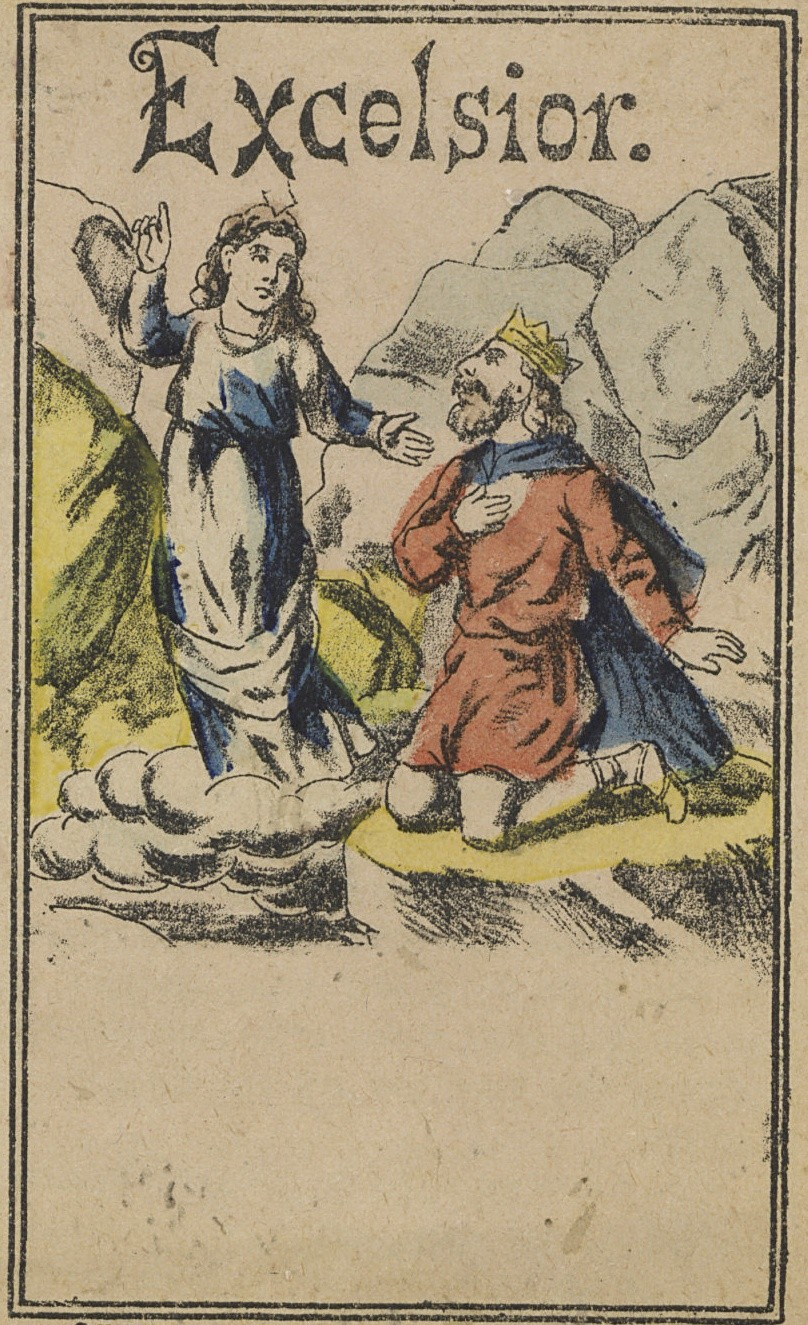
\includegraphics[height=4.6cm]{restoration_input_1_opt.jpg}
\vskip 0.1cm
\tiny \textit{A typical Colibri scan ($n=53,000+$): chemical decay, faded contrast, no modern photographic cues.}
\end{columns}
\end{frame}

\begin{frame}{1.1b What Object Detection on This Archive Actually Looks Like}
\centering
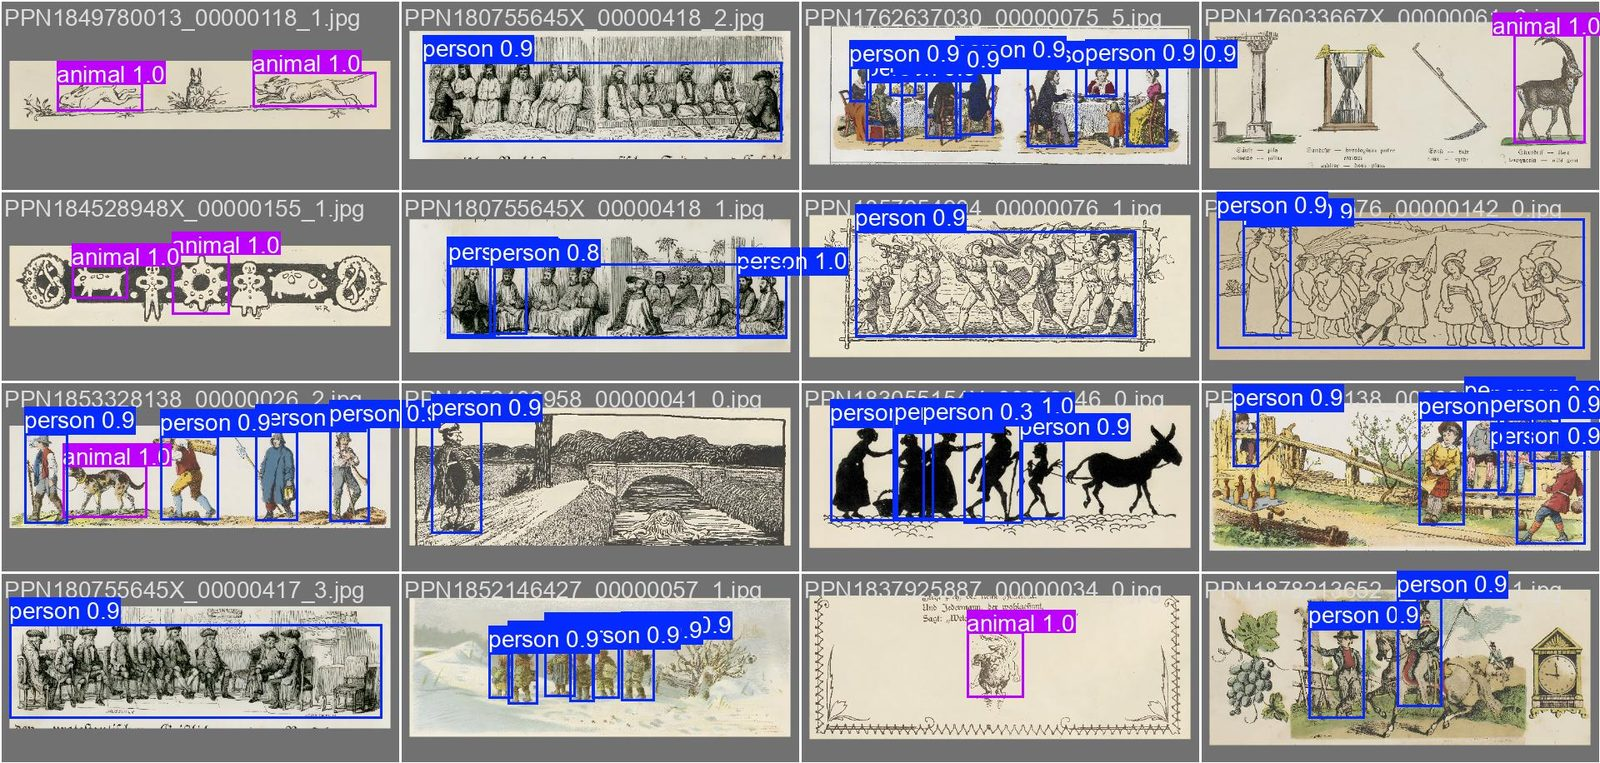
\includegraphics[width=0.90\textwidth]{yolo_detection_example_1.jpg}
\vskip 0.1cm
\scriptsize Real Tier 1 spatial-grounding output (YOLOv11-seg) on 16 real Colibri scans. Note the genuine failure modes: coarse two-class output (\texttt{person}/\texttt{animal}) and overlapping duplicate boxes on crowded scenes.
\end{frame}

\begin{frame}{1.2 Baselines, and Why They Are Not Enough}
\footnotesize
A detector this unreliable cannot be deployed without knowing \emph{which} of its predictions to trust. Three standard ways a single model could try to signal its own uncertainty, same error-detection task:
\begin{columns}[T]
\column{0.56\textwidth}
\centering
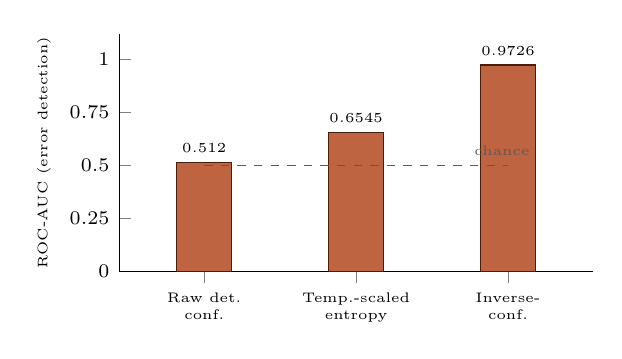
\begin{tikzpicture}
\begin{axis}[
  ybar, bar width=20pt, width=7.6cm, height=4.6cm,
  ymin=0, ymax=1.12, ylabel={ROC-AUC (error detection)}, ylabel style={font=\tiny},
  symbolic x coords={RawConf, Entropy, InvConf},
  xtick=data,
  xticklabels={{Raw det.\\conf.},{Temp.-scaled\\entropy},{Inverse-\\conf.}},
  x tick label style={font=\tiny, align=center},
  tick label style={font=\scriptsize}, axis lines*=left, enlarge x limits=0.28,
  nodes near coords, nodes near coords style={font=\tiny}, every node near coord/.append style={/pgf/number format/.cd, fixed, precision=4},
  axis line style={-}, ytick={0,0.25,0.5,0.75,1.0}
]
\addplot[fill=PrismOrange!85, draw=PrismOrange!40!black] coordinates {(RawConf, 0.5120) (Entropy, 0.6545) (InvConf, 0.9726)};
\draw[dashed, PrismGray] (axis cs:RawConf,0.5) -- (axis cs:InvConf,0.5) node[pos=0.98, above, font=\tiny, PrismGray] {chance};
\end{axis}
\end{tikzpicture}

\column{0.42\textwidth}
\begin{itemize}\footnotesize
  \item \textbf{Raw confidence}: box score, used directly -- barely better than a coin flip.
  \item \textbf{Entropy}: softmax entropy, single VLM -- weak.
  \item \textbf{Inverse-confidence}: $1-$conf., single pass -- strong discrimination, but badly overconfident (ECE $\approx0.19$).
\end{itemize}
\end{columns}
\begin{alertblock}{\scriptsize The Gap}
\scriptsize No single-model method is both discriminative \emph{and} well-calibrated.
\end{alertblock}
\end{frame}

\begin{frame}{1.3 The Contribution, and What It Does Not Claim}
\scriptsize
\begin{center}
\begin{tabular}{@{}p{1.9cm} p{10.2cm}@{}}
\toprule
\textbf{Task} & Index $53{,}000$ historical scans, no labelled training data --- and say which descriptions to trust. \\
\addlinespace
\textbf{Contribution} & Not a better detector: a \emph{routing} mechanism. Fuse four models into an uncertainty score, calibrate it, threshold it under a distribution-free risk bound. \\
\addlinespace
\textbf{Result} & \emph{Ties} the baselines on ranking errors --- said plainly rather than claimed as a win. Wins on \textbf{calibration} ($\text{ECE}<0.001$ vs $0.19$--$0.28$) and is the only one \textbf{certified}: $60.6\%$ auto-approved at $91.1\%$ recall (Slide 3.6). \\
\bottomrule
\end{tabular}
\end{center}
\vspace{-1mm}
\begin{alertblock}{\scriptsize What was withdrawn --- said up front}
\scriptsize The original claim was that \emph{disagreement} is what makes this work. It is not: a plain confidence baseline ties it (A.14), and that holds after running all four models on all $12{,}110$ images (A.24). The mechanism stands; the explanation does not.
\end{alertblock}
\end{frame}

\begin{frame}{1.4 Research Questions}
\scriptsize
\centering
\begin{table}[!htbp]
\begin{tabular}{p{3.2cm}p{9.0cm}}
\toprule
\textbf{RQ ID} & \textbf{Research Question} \\
\midrule
\textbf{RQ1: Disagreement Uncertainty} & Can cross-modal agent disagreement reliably estimate epistemic uncertainty on domain-shifted visual collections? \\
\textbf{RQ2: Workload Reduction} & Does the multi-agent framework reduce human curation workload without sacrificing error recall? \\
\textbf{RQ3: Complementarity \& Contradiction} & Does cross-modal contradiction detection improve curation precision beyond the Tier 1 SAA validation core alone? \\
\textbf{RQ4: Retrieval \& Transferability} & Can the framework support archival retrieval and cross-collection discovery? \\
\bottomrule
\end{tabular}
\end{table}
\end{frame}

\begin{frame}{1.5 Prior Work I: Detection on Historical Material}
\footnotesize
\begin{itemize}
  \setlength\itemsep{6pt}
  \item \textbf{Kim, Im and Mandl (2024)} --- the closest precedent. Translate modern labelled photographs into historical style (CycleGAN), then pseudo-label to expand supervision.
  \item \textbf{This thesis inverts the direction}: they adapt the \emph{training} distribution, we restore scans at \emph{inference}. Not a refutation --- it adds a validation their protocol lacks. Graded against its own teacher a pseudo-labelled student scores $\mathbf{0.989}$; graded against a person, $\mathbf{0.1462}$.
  \item \textbf{Lee (2013)} introduced pseudo-labelling; \textbf{Xie et al.\ (2020)} refined it as Noisy Student.
  \item \textbf{Both assume the pseudo-labels are roughly right.} On a degraded archive that assumption fails quietly --- the failure this thesis measures.
\end{itemize}
\end{frame}

\begin{frame}{1.6 Prior Work II: Uncertainty and Risk Control}
\footnotesize
\begin{itemize}
  \setlength\itemsep{6pt}
  \item \textbf{Seung, Opper and Sompolinsky (1992)} --- the idea this is built on: keep several hypotheses that all fit, treat their disagreements as the uncertain points.
  \item \textbf{Lakshminarayanan et al.\ (2017)} made it practical as deep ensembles; \textbf{Gal and Ghahramani (2016)} gave the cheap version (test-time dropout).
  \item \textbf{The difference here is what varies.} Ensemble members share an architecture and a corpus, so their mistakes stay correlated. Our four models share almost no training signal --- and we still report that this is not enough on images with no scene.
  \item \textbf{Kendall and Gal (2017)} separate reducible from inherent uncertainty; \textbf{Guo et al.\ (2017)} showed modern networks are badly calibrated.
  \item \textbf{Angelopoulos et al.\ (2024)} extend conformal prediction to any bounded loss --- what lets this thesis bound the rate of errors approved without review.
\end{itemize}
\end{frame}

\begin{frame}{1.7 Prior Work III: Zero-Shot Models and Cultural Heritage}
\footnotesize
\begin{itemize}
  \setlength\itemsep{6pt}
  \item \textbf{CLIP (2021)} aligned image and text encoders on 400M web pairs, so images can be classified against label \emph{text} with no training on those labels. \textbf{SigLIP (2023)}, deployed here, swaps the batch-wide softmax for a per-pair sigmoid, making it practical at corpus scale. \textbf{Grounding DINO (2023)} carries the same idea into detection.
  \item \textbf{Why it matters here}: a closed label set fixed at training time cannot represent categories archival scholarship is still arguing about.
  \item \textbf{Westlake et al.\ (2016)} showed photo-trained detectors degrade on artwork --- their PeopleArt data is the cross-style benchmark used here; \textbf{Schneider and Vollmer (2024)} show the same for pose.
  \item \textbf{Bengamra et al.\ (2024)} survey the recurring obstacles; \textbf{Impett and Offert (2022)} ask what it means, epistemically, to apply these models to art history at all.
\end{itemize}
\end{frame}

\section{How SAA Is Implemented}

\begin{frame}{2.1 A Quick Map: The Six Cohorts}
\scriptsize
\begin{columns}[T]
\column{0.47\textwidth}
\centering
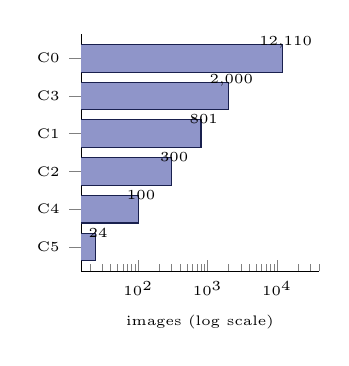
\begin{tikzpicture}
\begin{axis}[
  xbar, bar width=10pt, width=4.6cm, height=4.6cm,
  xmode=log, xmin=15, xmax=40000, xlabel={images ($\log$ scale)}, xlabel style={font=\tiny},
  symbolic y coords={C5,C4,C2,C1,C3,C0},
  ytick=data, y tick label style={font=\tiny}, tick label style={font=\tiny},
  axis lines*=left, enlarge y limits=0.13,
  nodes near coords, every node near coord/.append style={font=\tiny, xshift=1pt},
  point meta=explicit symbolic
]
\addplot[fill=PrismRed!55, draw=HildesheimRed!50!black] coordinates {
  (24,C5) [24] (100,C4) [100] (300,C2) [300] (801,C1) [801] (2000,C3) [2{,}000] (12110,C0) [12{,}110]};
\end{axis}
\end{tikzpicture}

\column{0.51\textwidth}
\vspace{-1mm}
{\tiny
\begin{tabular}{@{}p{0.7cm}p{6.0cm}@{}}
\textbf{$C_0$} & Everything the pipeline ran on. Deployment and indexing. \\[2pt]
\textbf{$C_3$} & $C_1$ plus $1{,}199$ catalogue records. The train / cal / test split. \\[2pt]
\textbf{$C_1$} & Expert-reviewed. Calibration and the headline $0.9724$. \\[2pt]
\textbf{$C_2$} & Bounding-box audit. The spatial error paradox. \\[2pt]
\textbf{$C_4$} & Frontier comparison and a routing simulation. \\[2pt]
\textbf{$C_5$} & Real Europeana images, 10 institutions. The transfer failure. \\
\end{tabular}}
\end{columns}
\vspace{-1mm}
\begin{alertblock}{\scriptsize Why this slide exists}
\scriptsize These answer \emph{different} questions and must not be pooled. The headline $0.9724$, the risk guarantee, the negative-control stress test and the transfer pilot each come from a different row --- which is exactly how the label-integrity failure of Slide 3.5 stayed hidden for so long.
\end{alertblock}
\end{frame}

\begin{frame}{2.2 The System, End to End}
\centering
{\scriptsize\color{PrismGray} DCV-MAC: a three-stage pipeline that runs cheap local models first, computes \emph{two} things from them --- a class prediction and an uncertainty estimate (hence ``dual-core'') --- and escalates only what it cannot resolve.}\\[0.3mm]
\resizebox{!}{4.4cm}{%
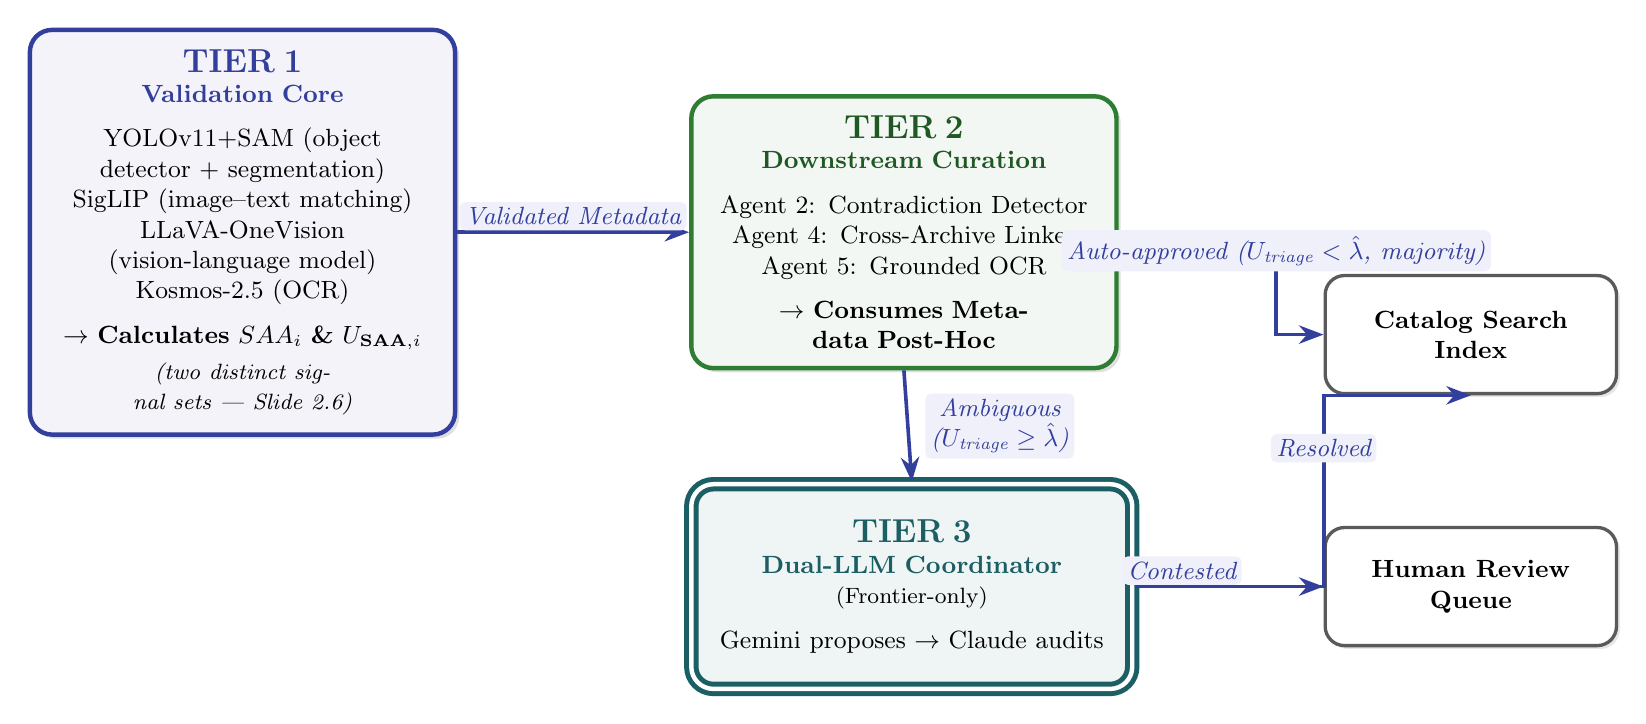
\begin{tikzpicture}[
  every node/.style={font=\small},
  tierbox1/.style={draw=HildesheimRed, line width=1.6pt, fill=HildesheimRed!6, rounded corners=8pt, align=center, minimum width=5.4cm, minimum height=3.6cm, text width=4.9cm, inner sep=7pt, drop shadow={shadow xshift=1.5pt, shadow yshift=-1.5pt, opacity=0.25}},
  tierbox2/.style={draw=PrismGreen, line width=1.6pt, fill=PrismGreen!6, rounded corners=8pt, align=center, minimum width=5.4cm, minimum height=3.2cm, text width=4.9cm, inner sep=7pt, drop shadow={shadow xshift=1.5pt, shadow yshift=-1.5pt, opacity=0.25}},
  coordbox/.style={draw=PrismBlue, line width=1.8pt, fill=PrismBlue!7, rounded corners=8pt, align=center, minimum width=5.6cm, minimum height=2.6cm, text width=5.0cm, inner sep=7pt, double, double distance=1.6pt, drop shadow={shadow xshift=1.5pt, shadow yshift=-1.5pt, opacity=0.25}},
  outbox/.style={draw=PrismGray, line width=1.2pt, fill=white, rounded corners=7pt, align=center, minimum width=3.7cm, minimum height=1.5cm, inner sep=5pt, drop shadow={shadow xshift=1.2pt, shadow yshift=-1.2pt, opacity=0.2}},
  arrow/.style={->, >=Stealth, thick, HildesheimRed, line width=1.3pt},
  flowlabel/.style={font=\small\itshape, align=center, fill=PrismLightBlue!60, inner sep=2pt, rounded corners=2pt}
]

\node[tierbox1] at (0,0) (t1) {%
  {\color{HildesheimRed}\bfseries\large TIER 1}\\
  {\color{HildesheimRed}\bfseries Validation Core}\\[5pt]
  YOLOv11+SAM (object detector + segmentation) \\ SigLIP (image--text matching) \\ LLaVA-OneVision (vision-language model) \\ Kosmos-2.5 (OCR)\\[5pt]
  {$\rightarrow$ \textbf{Calculates $SAA_i$ \& $U_{\text{SAA},i}$}}\\[2pt]
  {\footnotesize\itshape (two distinct signal sets --- Slide 2.6)}
};

\node[tierbox2] at (8.4,0) (t2) {%
  {\color{PrismGreen!70!black}\bfseries\large TIER 2}\\
  {\color{PrismGreen!70!black}\bfseries Downstream Curation}\\[5pt]
  Agent 2: Contradiction Detector \\ Agent 4: Cross-Archive Linker \\ Agent 5: Grounded OCR\\[5pt]
  {$\rightarrow$ \textbf{Consumes Metadata Post-Hoc}}
};

\node[outbox] at (15.6,-1.3) (index) {\textbf{Catalog Search}\\\textbf{Index}};

\node[coordbox] at (8.5,-4.5) (t3) {%
  {\color{PrismBlue}\bfseries\large TIER 3}\\
  {\color{PrismBlue}\bfseries Dual-LLM Coordinator}\\
  {\footnotesize (Frontier-only)}\\[5pt]
  Gemini proposes\ $\rightarrow$\ Claude audits
};

\node[outbox] at (15.6,-4.5) (hitl) {\textbf{Human Review}\\\textbf{Queue}};

\draw[arrow] (t1) -- (t2) node[midway, above, flowlabel] {Validated Metadata};
\draw[arrow] (t2.east) -- ++(2.0,0) |- (index.west) node[pos=0.2, above, flowlabel] {Auto-approved ($U_{\text{triage}} < \hat\lambda$, majority)};
\draw[arrow] (t2.south) -- (t3.north) node[midway, right, flowlabel, xshift=2mm] {Ambiguous\\($U_{\text{triage}} \ge \hat\lambda$)};
\draw[arrow] (t3.east) -- ++(2.4,0) |- (index.south) node[pos=0.32, above, flowlabel] {Resolved};
\draw[arrow] (t3.east) -- (hitl.west) node[pos=0.25, above, flowlabel] {Contested};
\end{tikzpicture}%
}

{\tiny\textit{Frontier-only: a local same-model variant caught 0/25 self-contradictions and was dropped (A.4).}}
\begin{block}{\tiny\textbf{Architectural Decoupling Rule}}
\tiny Tier 2 runs on post-validation metadata only, never feeds Tier 1's $SAA$, and \textbf{gates nothing} --- routing is decided at \emph{triage}.
\end{block}
\end{frame}

\begin{frame}{2.3 Why This Design?}
\footnotesize
\begin{columns}[T]
\column{0.49\textwidth}
\begin{block}{Why Three Stages, Not One Model}
Cheap and automatic first, expensive and human last. Each step only sees what the last one couldn't resolve -- that's what keeps the paid, slow steps rare.
\end{block}
\begin{block}{Why Tier 2 Runs Separately, After}
It only touches images Tier 1 already trusts, and only \emph{adds} value (links, inscriptions) -- it never gets a vote on trust itself.
\end{block}

\column{0.49\textwidth}
\begin{block}{Why Frontier-Only for Tier 3}
We tried a free, local ``second opinion'' first: same model critiquing itself. It caught \textbf{0 of 25} real self-contradictions -- same weights just agree with themselves. Genuinely different local models did catch real errors when retested later -- but the critique itself wasn't always trustworthy either (A.4). So Tier 3 uses two paid frontier models instead, only for the small, hard fraction everything else couldn't resolve.
\end{block}
\end{columns}
\end{frame}

\begin{frame}{2.4 Tier 1 Validation Core (4-Model Ensemble)}
\footnotesize
\begin{columns}[T]
\column{0.48\textwidth}
\begin{block}{Looking at Objects and Scenes}
\begin{itemize}
  \item \textbf{YOLOv11-seg + SAM} answers \emph{where things are}: boxes and instance masks. In the deployed run the scalar $A_i^{\text{object}}$ was not taken from it --- see A.14.
  \item \textbf{SigLIP} answers \emph{what kind of scene this is} overall, scoring the image against the institution's own category names ($A_i^{\text{scene}}$).
\end{itemize}
\end{block}

\column{0.48\textwidth}
\begin{block}{Reading the Image and Its Text}
\begin{itemize}
  \item \textbf{LLaVA-OneVision 7B} answers \emph{what is happening here}, in words -- a description and a list of what it thinks it sees ($A_i^{\text{vlm}}$).
  \item \textbf{Kosmos-2.5} answers \emph{what does it say}: text pinned to the spot in the image where it appears ($A_i^{\text{ocr}}$).
\end{itemize}
\end{block}
\end{columns}
\end{frame}

\begin{frame}{2.5 Tier 2 Downstream Curation Agents}
\scriptsize
\begin{center}
\begin{tabular}{@{}p{2.4cm} p{9.6cm}@{}}
\toprule
\textbf{Agent 2}\newline Contradiction & The VLM mentions something the detector never found (``horse'' with no horse box) $\rightarrow$ flag for review. \\
\addlinespace
\textbf{Agent 4}\newline Cross-Archive Linker & Finds visually similar images across \emph{different} publication volumes --- the same motif recurring years apart. \\
\addlinespace
\textbf{Agent 5}\newline Grounded OCR & Reads inscriptions and captions, and ties each piece of text to \emph{where} it sits in the image. \\
\bottomrule
\end{tabular}
\end{center}
\vspace{1mm}
\begin{alertblock}{\scriptsize They curate --- they never judge trust}
\scriptsize All three run \emph{after} $SAA_i$ and feed nothing back into it, so nothing here can change how much an image is trusted (the Decoupling Rule, Slide 2.2). How often each is actually right: Slide 3.7.
\end{alertblock}
\end{frame}

\begin{frame}{2.6 The Four Levels, and What Each Is For}
\centering
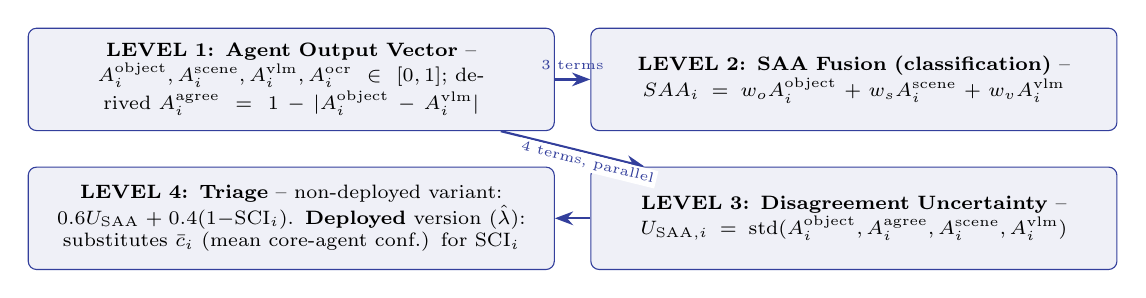
\begin{tikzpicture}[
  node distance=0.45cm and 0.45cm,
  every node/.style={font=\scriptsize},
  levelbox/.style={draw=HildesheimRed, fill=PrismRed!8, rounded corners=3pt, align=center, text width=6.4cm, minimum height=1.3cm, inner sep=4pt},
  arrow/.style={->, >=Stealth, thick, HildesheimRed}
]
\node[levelbox] (l1) {\textbf{LEVEL 1: Agent Output Vector} -- $A_i^{\text{object}}, A_i^{\text{scene}}, A_i^{\text{vlm}}, A_i^{\text{ocr}} \in [0,1]$; derived $A_i^{\text{agree}} = 1-|A_i^{\text{object}}-A_i^{\text{vlm}}|$};
\node[levelbox, right=of l1] (l2) {\textbf{LEVEL 2: SAA Fusion (classification)} -- $SAA_i = w_o A_i^{\text{object}} + w_s A_i^{\text{scene}} + w_v A_i^{\text{vlm}}$};
\node[levelbox, below=of l2] (l3) {\textbf{LEVEL 3: Disagreement Uncertainty} -- $U_{\text{SAA}, i} = \operatorname{std}(A_i^{\text{object}}, A_i^{\text{agree}}, A_i^{\text{scene}}, A_i^{\text{vlm}})$};
\node[levelbox, below=of l1] (l4) {\textbf{LEVEL 4: Triage} -- non-deployed variant: $0.6U_{\text{SAA}} + 0.4(1{-}\text{SCI}_i)$. \textbf{Deployed} version ($\hat\lambda$): substitutes $\bar{c}_i$ (mean core-agent conf.) for $\text{SCI}_i$};

\draw[arrow] (l1) -- (l2) node[midway, above, font=\tiny] {3 terms};
\draw[arrow] (l1) -- (l3) node[pos=0.62, below, sloped, font=\tiny, fill=white, inner sep=1pt] {4 terms, parallel};
\draw[arrow] (l3) -- (l4);
\end{tikzpicture}

\vspace{1mm}
\begin{center}\tiny
\begin{tabular}{@{}l l l l@{}}
\toprule
& \textbf{The question} & \textbf{Signals} & \textbf{Operator} \\
\midrule
\textbf{L1} Agents & Can four models be compared? & --- & normalise to $[0,1]$ \\
\textbf{L2} $SAA$ & \emph{What} is in the image? & Obj, Scene, VLM & weighted mean \\
\textbf{L3} $U_{\text{SAA}}$ & \emph{Trust} that answer? & Obj, \textbf{Agree}, Scene, VLM & std \\
\textbf{L4} Triage & \emph{Who sees} it? & $U_{\text{SAA}}$ + confidence & $0.6\sigma+0.4(1{-}\bar c)$ \\
\bottomrule
\end{tabular}
\end{center}
\vspace{-1mm}
\begin{alertblock}{\scriptsize The one thing to carry forward}
\scriptsize L2 decides the answer; L3 decides whether to believe it. Different equations over different signals --- so $U_{\text{SAA}} \neq 1-SAA$. Agreement is \textbf{derived}, not a fourth model (A.14).
\end{alertblock}
\end{frame}

\section{Experimental Results}

\begin{frame}{3.1 What Happens When a Model Grades Its Own Work}
\scriptsize
\begin{columns}[T]
\column{0.50\textwidth}
\begin{block}{Where We Started: Nothing Works}
Point YOLOv11 (COCO-trained) straight at un-restored grayscale scans ($C_0$) and it finds essentially nothing:
\begin{itemize}
    \item \textbf{mAP50 (raw scans)}: \evidence{0.0047}
    \item \textbf{Precision (raw scans)}: \evidence{0.0081}
    \item \textbf{Recall (raw scans)}: \evidence{0.0283}
\end{itemize}
\end{block}

\begin{block}{The Trap: It Looked Like We Fixed It}
Train a student detector on the teacher's own pseudo-labels, and the score looks superb -- until a human checks the same model's work:
\begin{itemize}
    \item \textbf{Graded against its teacher}: \textbf{0.989} mAP50
    \item \textbf{Graded against a human ($C_2, n=300$)}: \evidence{\textbf{0.1462}}
\end{itemize}
\end{block}

\column{0.46\textwidth}
\centering
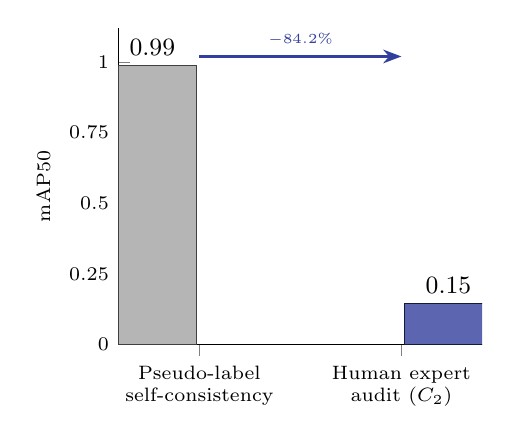
\begin{tikzpicture}
\begin{axis}[
  ybar, bar width=32pt, width=6.2cm, height=5.6cm,
  ymin=0, ymax=1.12, ylabel={mAP50}, ylabel style={font=\scriptsize},
  symbolic x coords={PL,Human},
  xtick={PL,Human}, xticklabels={{Pseudo-label\\self-consistency},{Human expert\\audit ($C_2$)}},
  x tick label style={font=\scriptsize, align=center},
  tick label style={font=\scriptsize}, axis lines*=left, enlarge x limits=0.4,
  nodes near coords, every node near coord/.append style={font=\small\bfseries},
  ytick={0,0.25,0.5,0.75,1.0}
]
\addplot[fill=PrismGray!45, draw=PrismGray!70!black] coordinates {(PL,0.989)};
\addplot[fill=HildesheimRed!80, draw=HildesheimRed!40!black] coordinates {(Human,0.1462)};
\draw[->, >=Stealth, thick, HildesheimRed] (axis cs:PL,1.02) -- (axis cs:Human,1.02) node[midway, above, font=\tiny, HildesheimRed] {$-84.2\%$};
\end{axis}
\end{tikzpicture}
\vskip 0.1cm
\tiny \textit{Same distilled student detector, two ground truths. The 84.2\% relative drop is the paradox.}
\end{columns}
\end{frame}
\begin{frame}{3.2 Head-to-Head: SAA vs.\ Every Baseline}
\footnotesize
\centering
All methods, same error-detection task, same expert cohort ($C_1$, $n=801$) -- SAA ties on discrimination and improves by more than two orders of magnitude on calibration:
\begin{center}
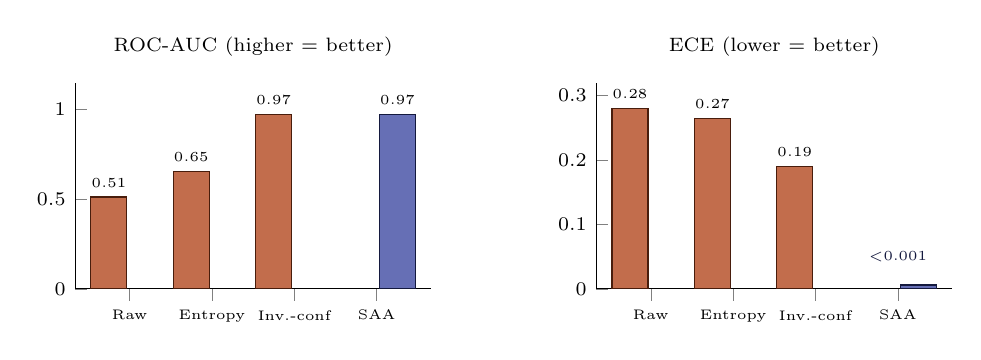
\begin{tikzpicture}
\begin{groupplot}[
  group style={group size=2 by 1, horizontal sep=2.1cm},
  width=6.1cm, height=4.2cm,
  symbolic x coords={Raw, Ent, Inv, SAA},
  xtick={Raw,Ent,Inv,SAA}, xticklabels={{Raw},{Entropy},{Inv.-conf},{SAA}},
  x tick label style={font=\tiny, align=center, rotate=0},
  tick label style={font=\scriptsize}, axis lines*=left, enlarge x limits=0.22,
  nodes near coords style={font=\tiny},
]
\nextgroupplot[ybar, bar width=13pt, title={\scriptsize ROC-AUC (higher = better)}, ymin=0, ymax=1.15, ytick={0,0.5,1}]
\addplot[fill=PrismOrange!80, draw=PrismOrange!40!black, nodes near coords] coordinates {(Raw,0.5120) (Ent,0.6545) (Inv,0.9726)};
\addplot[fill=HildesheimRed!75, draw=HildesheimRed!40!black, nodes near coords] coordinates {(SAA,0.9724)};

\nextgroupplot[ybar, bar width=13pt, title={\scriptsize ECE (lower = better)}, ymin=0, ymax=0.32, ytick={0,0.1,0.2,0.3}]
\addplot[fill=PrismOrange!80, draw=PrismOrange!40!black, nodes near coords] coordinates {(Raw,0.28) (Ent,0.265) (Inv,0.19)};
\addplot[fill=HildesheimRed!75, draw=HildesheimRed!40!black] coordinates {(SAA,0.006)};
\node[font=\tiny, HildesheimRed!40!black] at (axis cs:SAA,0.05) {$<$0.001};
\end{groupplot}
\end{tikzpicture}
\end{center}
\begin{alertblock}{\scriptsize The Result, Stated Plainly}
\scriptsize SAA ties the strongest baseline on discrimination (\evidence{0.9724 vs.\ 0.9726}) at the same single-pass cost; its advantage here is calibration. Two limits, both tested and reported: do the models agree confidently and wrongly on blank scenes (3.6)? And is \emph{disagreement} doing the work -- plain confidence ties it at \evidence{0.9717} (A.14)?
\end{alertblock}
\end{frame}
\begin{frame}{3.3 How Correlated Are the Four Agents?}
\footnotesize
Disagreement only works as a signal if the four models can actually disagree -- if they always moved in lockstep, there'd be nothing to measure. This matrix checks that assumption directly, across the full deployment corpus:
\begin{columns}[T]
\column{0.46\textwidth}
\centering
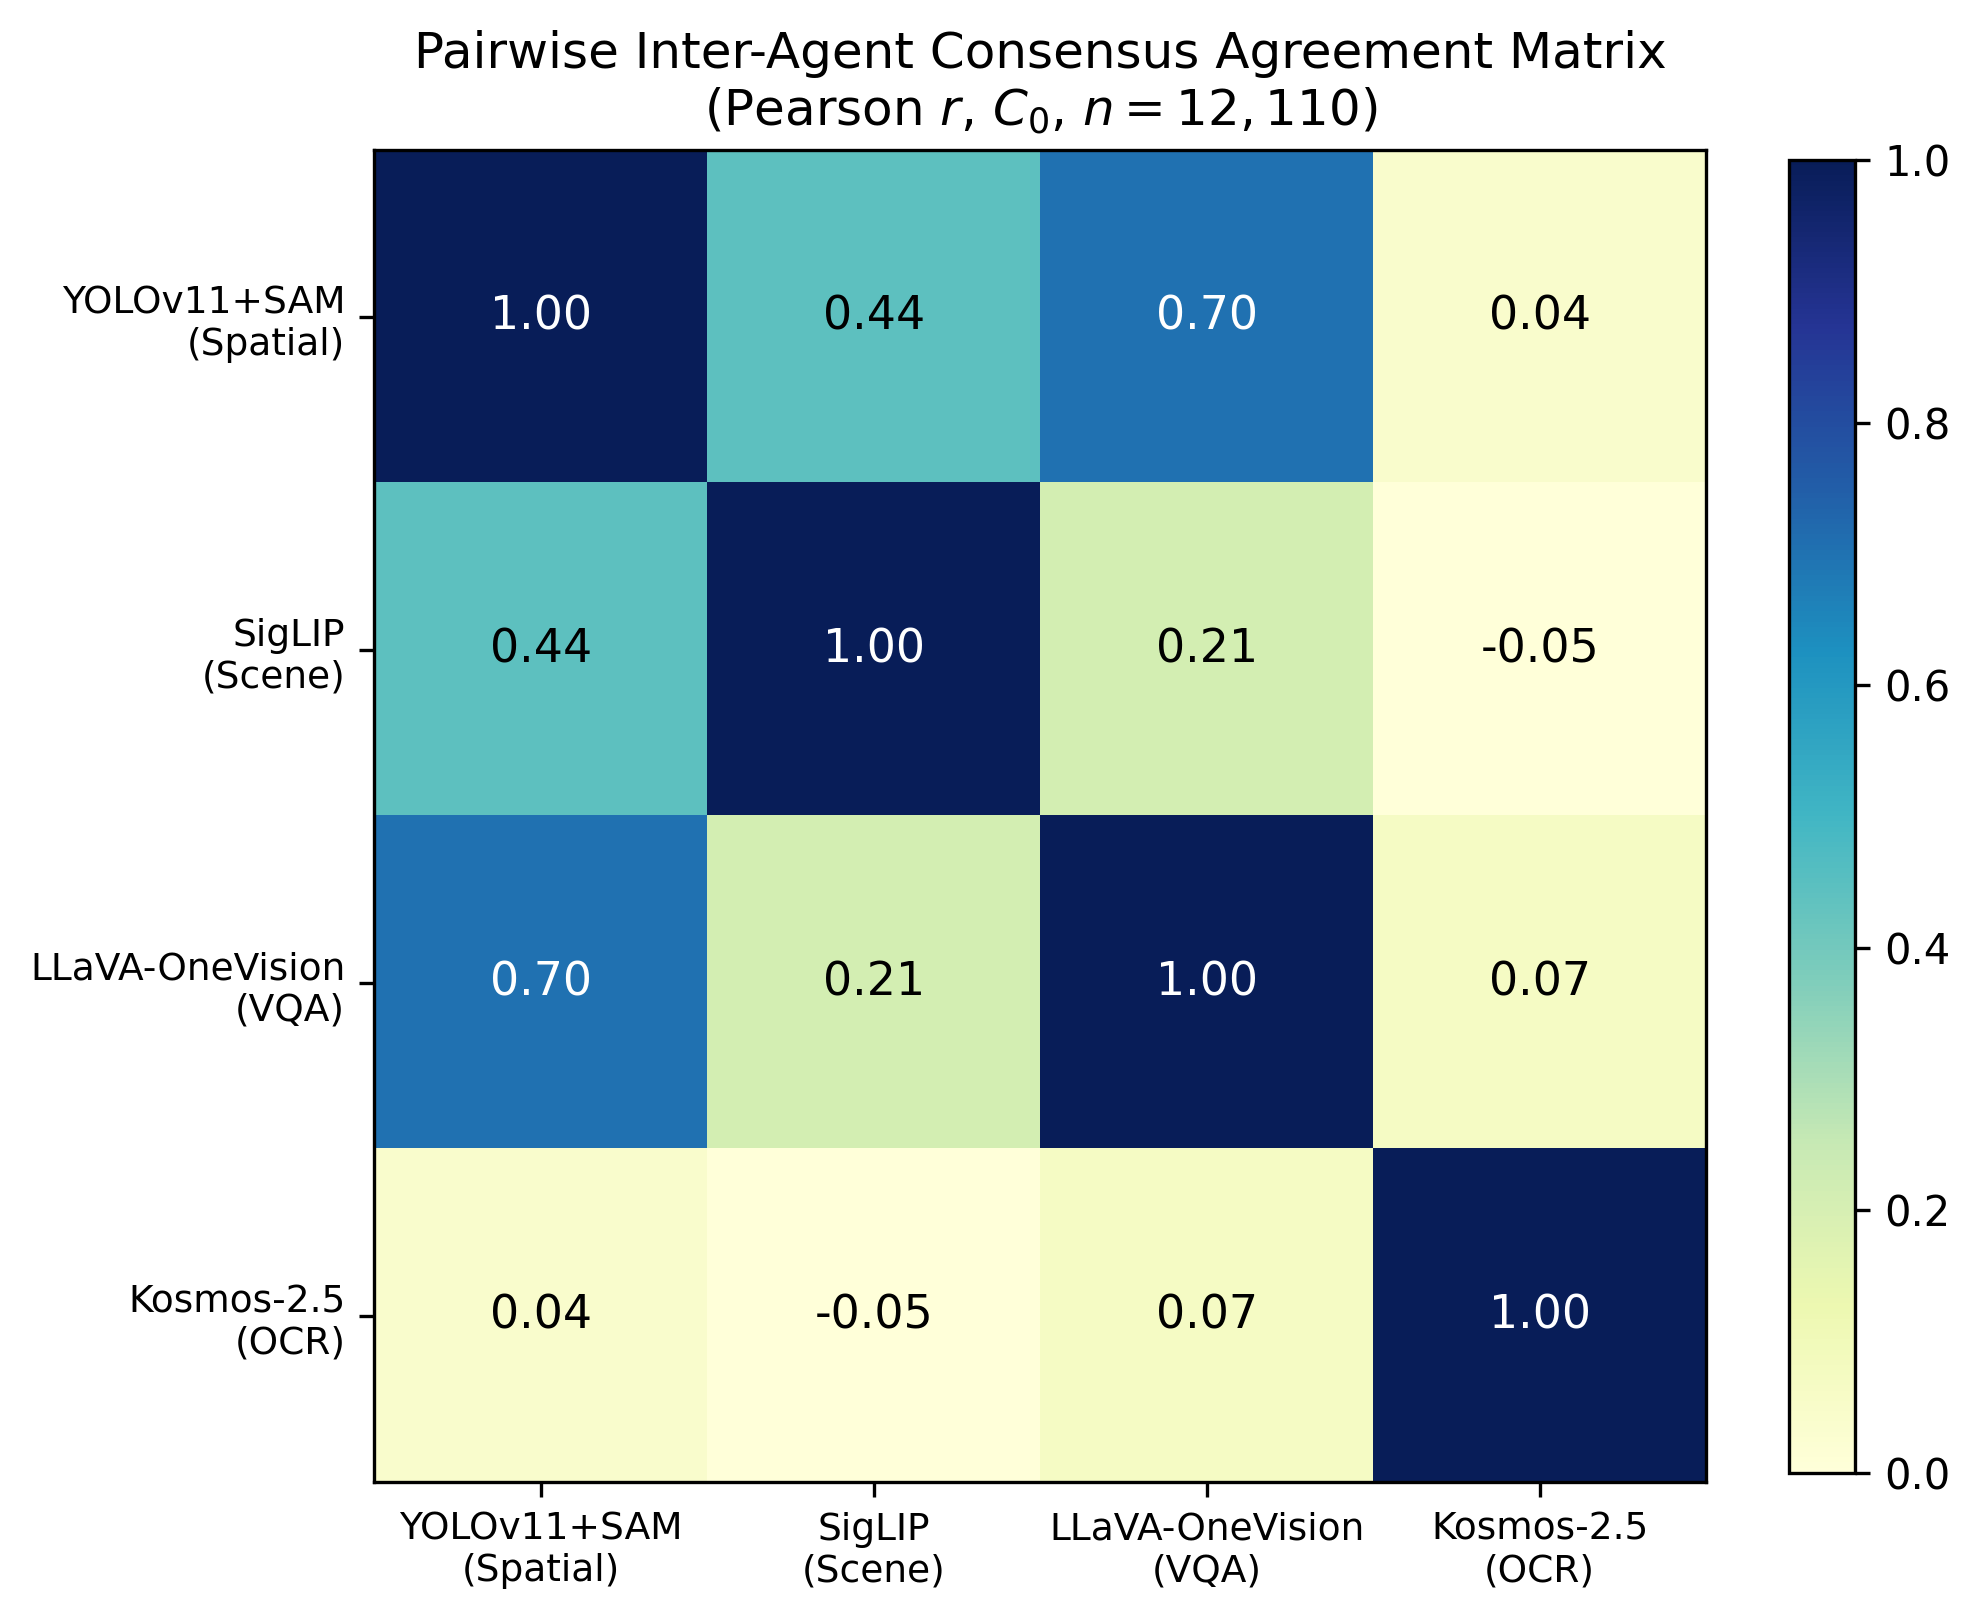
\includegraphics[width=\textwidth]{pairwise_agreement_heatmap_v9.png}
\vskip 0.1cm
\tiny \textit{Pairwise Inter-Agent Consensus Agreement Matrix (4 deployed Tier 1 agents, $C_0$, $n{=}12{,}110$).}

\column{0.50\textwidth}
\begin{block}{What It Shows}
Spatial grounding and VQA move together most closely ($r=0.70$) -- both are, in different ways, reading what objects are in the scene. Grounded OCR is the outlier ($r\le0.07$ against every other agent): reading text tells you something the other three simply can't see. That independence is exactly why removing OCR (Slide 3.4) hurts disagreement the most.
\end{block}
\end{columns}
\end{frame}
\begin{frame}{3.4 Tier 1 Agent Ablation: Which Model Drives Disagreement?}
\footnotesize
A different question from \S3.3: not which agents move together, but which one the disagreement signal would most miss. Drop each in turn, full corpus ($C_0$, $n{=}12{,}110$):

\begin{columns}[T]
\column{0.54\textwidth}
\centering
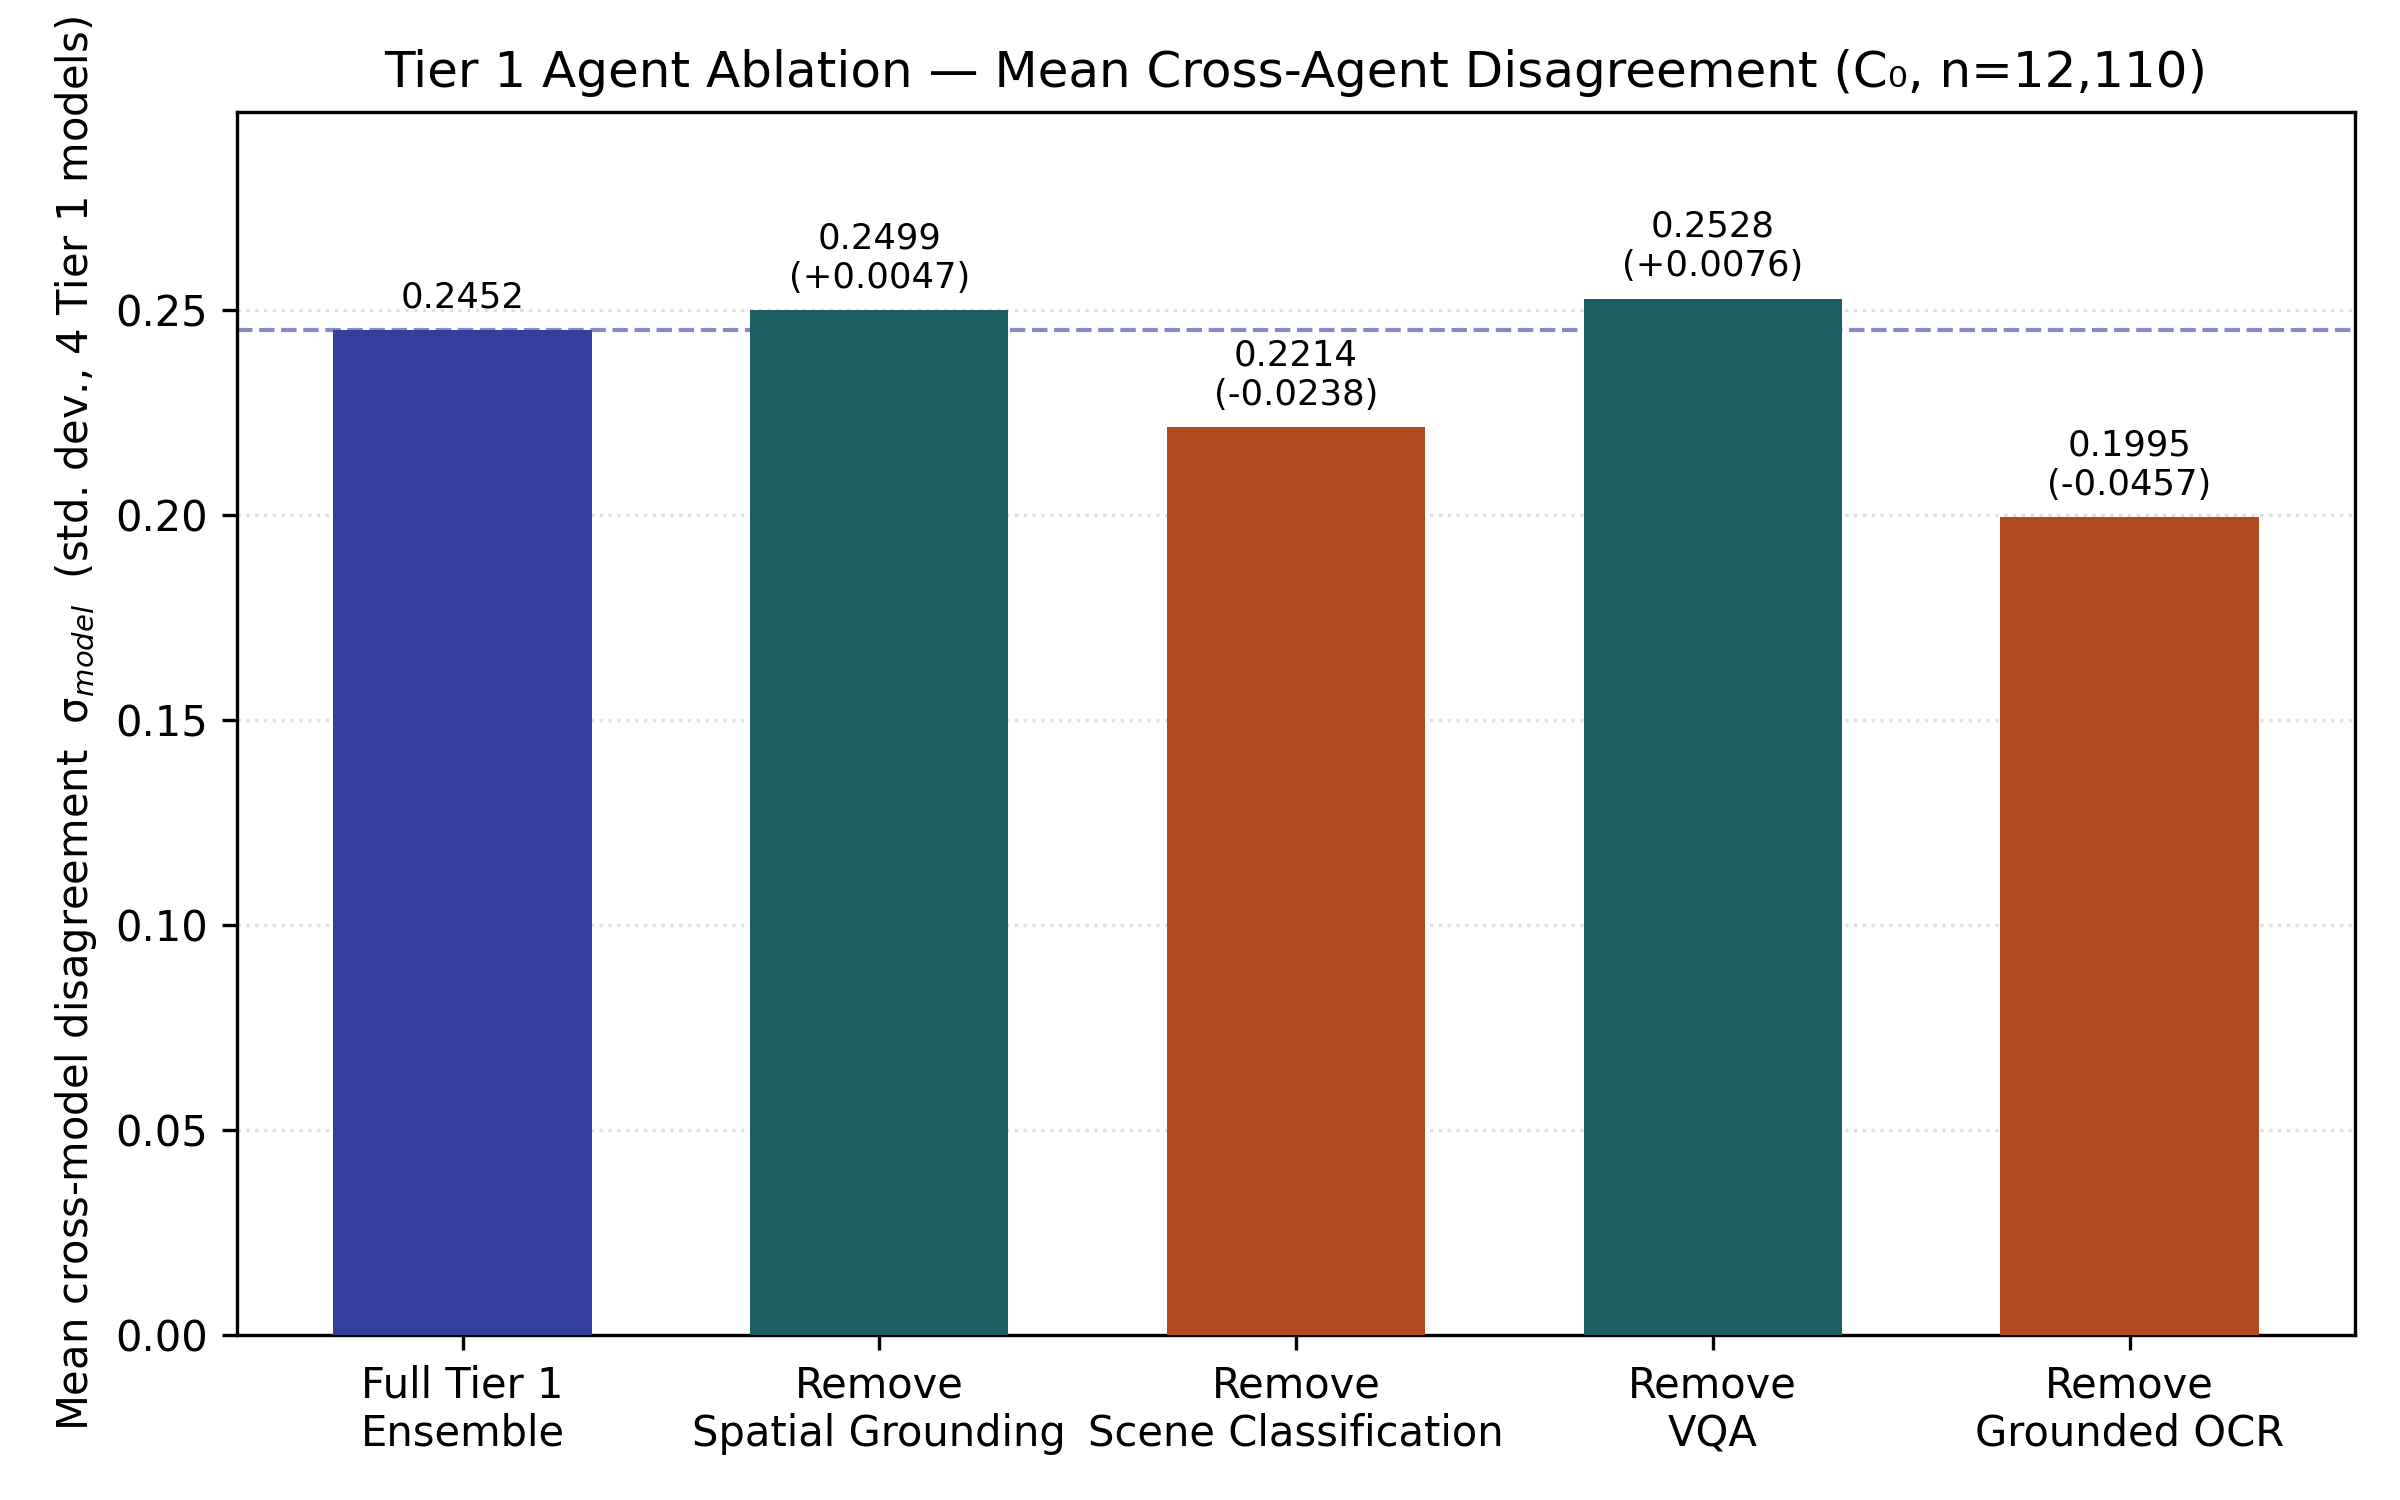
\includegraphics[width=\textwidth]{tier1_ablation_figure.png}

\column{0.44\textwidth}
\scriptsize
\begin{tabular}{lc}
\toprule
\textbf{Ablated} & $\sigma$ ($\Delta$) \\
\midrule
\textbf{Full ensemble} & \textbf{0.2452} (---) \\
Remove Spatial (YOLO) & 0.2499 ($+0.0047$) \\
Remove Scene (SigLIP) & 0.2214 ($-0.0238$) \\
Remove VQA (LLaVA) & 0.2528 ($+0.0076$) \\
Remove OCR (Kosmos) & \textbf{0.1995 ($-0.0457$)} \\
\bottomrule
\end{tabular}
\end{columns}

\end{frame}
\begin{frame}{3.5 Stress-Testing SAA: A Data Bug, Found and Fixed}
\scriptsize
A claim is only trustworthy once you have tested where it breaks --- and checked the test data is real.
\begin{columns}[T]
\column{0.5\textwidth}
\centering
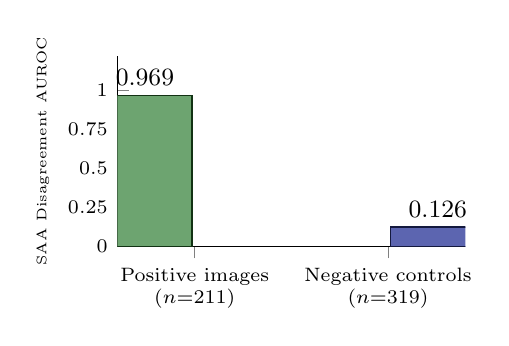
\begin{tikzpicture}
\begin{axis}[
  ybar, bar width=34pt, width=6.0cm, height=4.0cm,
  ymin=0, ymax=1.22, ylabel={SAA Disagreement AUROC}, ylabel style={font=\tiny},
  symbolic x coords={Pos,Neg},
  xtick={Pos,Neg}, xticklabels={{Positive images\\($n{=}211$)},{Negative controls\\($n{=}319$)}},
  x tick label style={font=\scriptsize, align=center},
  tick label style={font=\scriptsize}, axis lines*=left, enlarge x limits=0.4,
  nodes near coords, every node near coord/.append style={font=\small\bfseries, /pgf/number format/.cd, fixed, precision=3},
  ytick={0,0.25,0.5,0.75,1.0}
]
\addplot[fill=PrismGreen!70, draw=PrismGreen!40!black] coordinates {(Pos,0.9687)};
\addplot[fill=HildesheimRed!80, draw=HildesheimRed!40!black] coordinates {(Neg,0.1259)};
\end{axis}
\end{tikzpicture}
\column{0.44\textwidth}
\begin{itemize}\scriptsize
  \item Positive images: the uncertainty score \textbf{ranks} the pipeline's errors cleanly.
  \item The $319$ negative controls we've now confirmed as real: disagreement still \textbf{misses} them, well below chance. \emph{Why below chance and not merely low --- A.19.}
\end{itemize}
\end{columns}

\vspace{-4.5mm}
\begin{alertblock}{\scriptsize Why the Numbers Here Changed --- Twice}
\scriptsize $241$ images were labelled ``no scene'' by no one --- the first test measured bad labels. Hand-review left $38$ real negatives: the finding survived, but on $5$ errors. A third pass reviewed $285$ more; on the $123$ new negatives \emph{alone}, $0.1852$, again below chance. Pooled: $\mathbf{0.1259}$, $n{=}319$, $50$ errors, CI $[0.062,0.196]$ --- \textbf{replicated on data that played no part in producing it.}
\end{alertblock}
\end{frame}
\begin{frame}{3.6 A Guarantee on How Many Errors Get Through}
\scriptsize
\begin{columns}[T]
\column{0.58\textwidth}
\centering
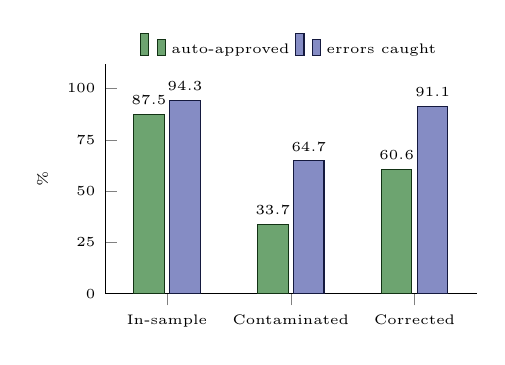
\begin{tikzpicture}
\begin{axis}[
  ybar, bar width=11pt, width=6.3cm, height=4.5cm,
  ymin=0, ymax=112, ylabel={\%}, ylabel style={font=\tiny},
  symbolic x coords={In-sample,Contaminated,Corrected},
  xtick=data, x tick label style={font=\tiny, align=center},
  tick label style={font=\tiny}, axis lines*=left, enlarge x limits=0.25,
  nodes near coords, every node near coord/.append style={font=\tiny},
  legend style={font=\tiny, at={(0.5,1.16)}, anchor=north, legend columns=2, draw=none},
  ytick={0,25,50,75,100}
]
\addplot[fill=PrismGreen!70, draw=PrismGreen!40!black]
  coordinates {(In-sample,87.5) (Contaminated,33.7) (Corrected,60.6)};
\addplot[fill=HildesheimRed!60, draw=HildesheimRed!40!black]
  coordinates {(In-sample,94.3) (Contaminated,64.7) (Corrected,91.1)};
\legend{auto-approved, errors caught}
\end{axis}
\end{tikzpicture}
\vskip 1pt
{\tiny Bound satisfied: \textcolor{PrismGreen!60!black}{\textbf{yes}} / \textcolor{HildesheimRed}{\textbf{no}} / \textcolor{PrismGreen!60!black}{\textbf{yes}}}

\column{0.40\textwidth}
{\color{PrismGray}\tiny Conformal Risk Control picks a threshold with a distribution-free upper bound on the error rate. The bound assumes nothing about data shape, but is only as good as the calibration set's match to deployment.}
\vskip 3pt
\begin{alertblock}{\scriptsize The deployed result}
\tiny $\hat\lambda=0.372$, risk $\mathcal{R}=0.0201\le0.05$, $\mathbf{2.31\times}$ lift over random review. \textbf{Every workload claim rests on this column.}
\end{alertblock}
\vspace{-2mm}
\begin{block}{\scriptsize The middle bar is the lesson}
\tiny The same procedure, unchanged, on a pool whose labels were $57.5\%$ wrong. The method did not fail --- the evaluation data did.
\end{block}
\end{columns}
\end{frame}
\begin{frame}{3.7 Do the Curation Agents Earn Their Place?}
\scriptsize
\begin{columns}[T]
\column{0.56\textwidth}
\centering
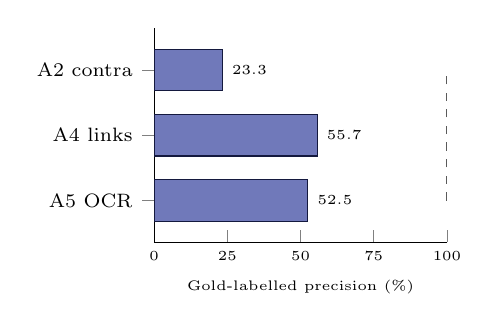
\begin{tikzpicture}
\begin{axis}[
  xbar, bar width=15pt, width=5.3cm, height=4.3cm,
  xmin=0, xmax=100, xlabel={Gold-labelled precision (\%)}, xlabel style={font=\tiny},
  symbolic y coords={A5 OCR,A4 links,A2 contra},
  ytick=data, y tick label style={font=\scriptsize}, tick label style={font=\tiny},
  axis lines*=left, enlarge y limits=0.32,
  nodes near coords, every node near coord/.append style={font=\tiny\bfseries},
  xtick={0,25,50,75,100}
]
\addplot[fill=HildesheimRed!70, draw=HildesheimRed!40!black]
  coordinates {(23.3,A2 contra) (55.7,A4 links) (52.5,A5 OCR)};
\draw[dashed, PrismGray] (axis cs:100,A5 OCR) -- (axis cs:100,A2 contra);
\end{axis}
\end{tikzpicture}
\vskip 1pt
{\tiny Agent 4 reaches $100\%$ above similarity $0.92$ --- a usable threshold.}

\column{0.42\textwidth}
\begin{block}{\scriptsize What this means}
\tiny None of the three feeds $U_{\text{SAA}}$ or any headline claim. They enrich the catalogue, and on gold labels none is reliable enough to act on unchecked.
\end{block}
\vspace{-2mm}
\begin{block}{\scriptsize Why no Tier 2 ablation}
\tiny They have \emph{no causal path} to any result here, so ablating them would move nothing. The right test for a curation aid is its precision when a human acts on it --- the chart.
\end{block}
\vspace{-2mm}
\begin{alertblock}{\scriptsize Retrieval (10-query pilot)}
\tiny P@10 $1.000$ vs $0.180$ keyword. Relevance labels share agent scores with the ranker: supporting evidence, not a benchmark.
\end{alertblock}
\end{columns}
\end{frame}

\section{Conclusion \& Future Work}

\begin{frame}{4.1 What This Thesis Establishes}
\footnotesize
\begin{enumerate}
    \setlength\itemsep{8pt}
    \item A model cannot grade itself. A detector trained on another model's guesses looked almost perfect --- but only when its own teacher marked the work. Measured against a person, most of that accuracy was not there.
    \item The archive can be told which descriptions to trust. The pipeline produces an uncertainty score, calibrated so its confidence means something, with a certified limit on how many errors slip through unchecked. Most images are catalogued automatically; the rest go to a person.
    \item The reason it works is not the reason we assumed. The score was built on the idea that disagreement between models reveals uncertainty. A plain confidence measure does just as well --- and nine different ways of measuring disagreement were tried before accepting that. The method stands; the explanation does not.
    \item Where it stops working is documented, not hidden. On images that truly show no scene, every model is confidently wrong together. Moved to a different archive the pipeline fails --- and a cheap check now predicts that before any labelling begins.
\end{enumerate}
\end{frame}

\begin{frame}{4.2 Future Work}
\footnotesize
\begin{itemize}
  \setlength\itemsep{4pt}
  \item Carry a second archive end to end, no-scene images included. Every result here comes from one collection, so nothing yet shows the method survives a change of institution, cataloguing practice or scanning equipment. Generality is so far an assumption, not a finding.
  \item Finish annotating the negative-control pool. A third pass took it from $38$ confirmed negatives to $319$ and replicated the blank-image result independently; $465$ images remain, and completing them would tighten the estimate further.
  \item Widen the interventional ablation. Removing one agent at a time already shows which the signal depends on; extending that to pairs is compute rather than new research.
  \item Collect real relevance judgements from an archivist, replacing the proxy labels behind the retrieval result.
  \item Test disagreement under a design that could falsify it: an ensemble whose members share no fusion formula, scored against a label not derived from the agents. This is the one item more labelling cannot settle: the present setup makes the answer partly circular.
\end{itemize}
\end{frame}

\begin{frame}
\centering
\vskip 0.4cm
{\large The most important result is not that the models became reliable.}
\vskip 0.6cm
{\Large\bfseries For an archive, knowing when to ask a person\\[0.15cm] is worth more than assuming the model is right.}
\vskip 0.9cm
\Large\textbf{Thank you}
\vskip 0.3cm
\small\textit{Questions \& discussion}
\end{frame}

\section*{Appendix / Backup Slides}

\begin{frame}{A.1 Generative Restoration Layer \& Axiom of Archival Integrity}
\scriptsize
\begin{columns}[T]
\column{0.50\textwidth}
\begin{block}{Three-Stage Generative Pipeline}
Raw scans ($\mathbf{I}_{\text{raw}}$) undergo:
\begin{enumerate}
    \item CycleGAN Grayscale-to-Color Translation
    \item Real-ESRGAN $4\times$ Super-Resolution
    \item Stable Diffusion Img2Img ($\text{strength}=0.35$)
\end{enumerate}
Yields $+0.052$ mAP gain (end-to-end vs.\ raw scans, same detector) and increases sharpness on $83.8\%$ of scans.
\end{block}

\begin{alertblock}{\textbf{The Axiom of Archival Integrity}}
The AI-restored image ($\mathbf{I}_{\text{refined}}$) is strictly an internal visual token translation layer for model feature alignment. It is NEVER stored or presented as primary archival evidence. All catalog metadata anchors strictly back to original digitized scans ($\mathbf{I}_{\text{raw}}$).
\end{alertblock}

\column{0.46\textwidth}
\centering
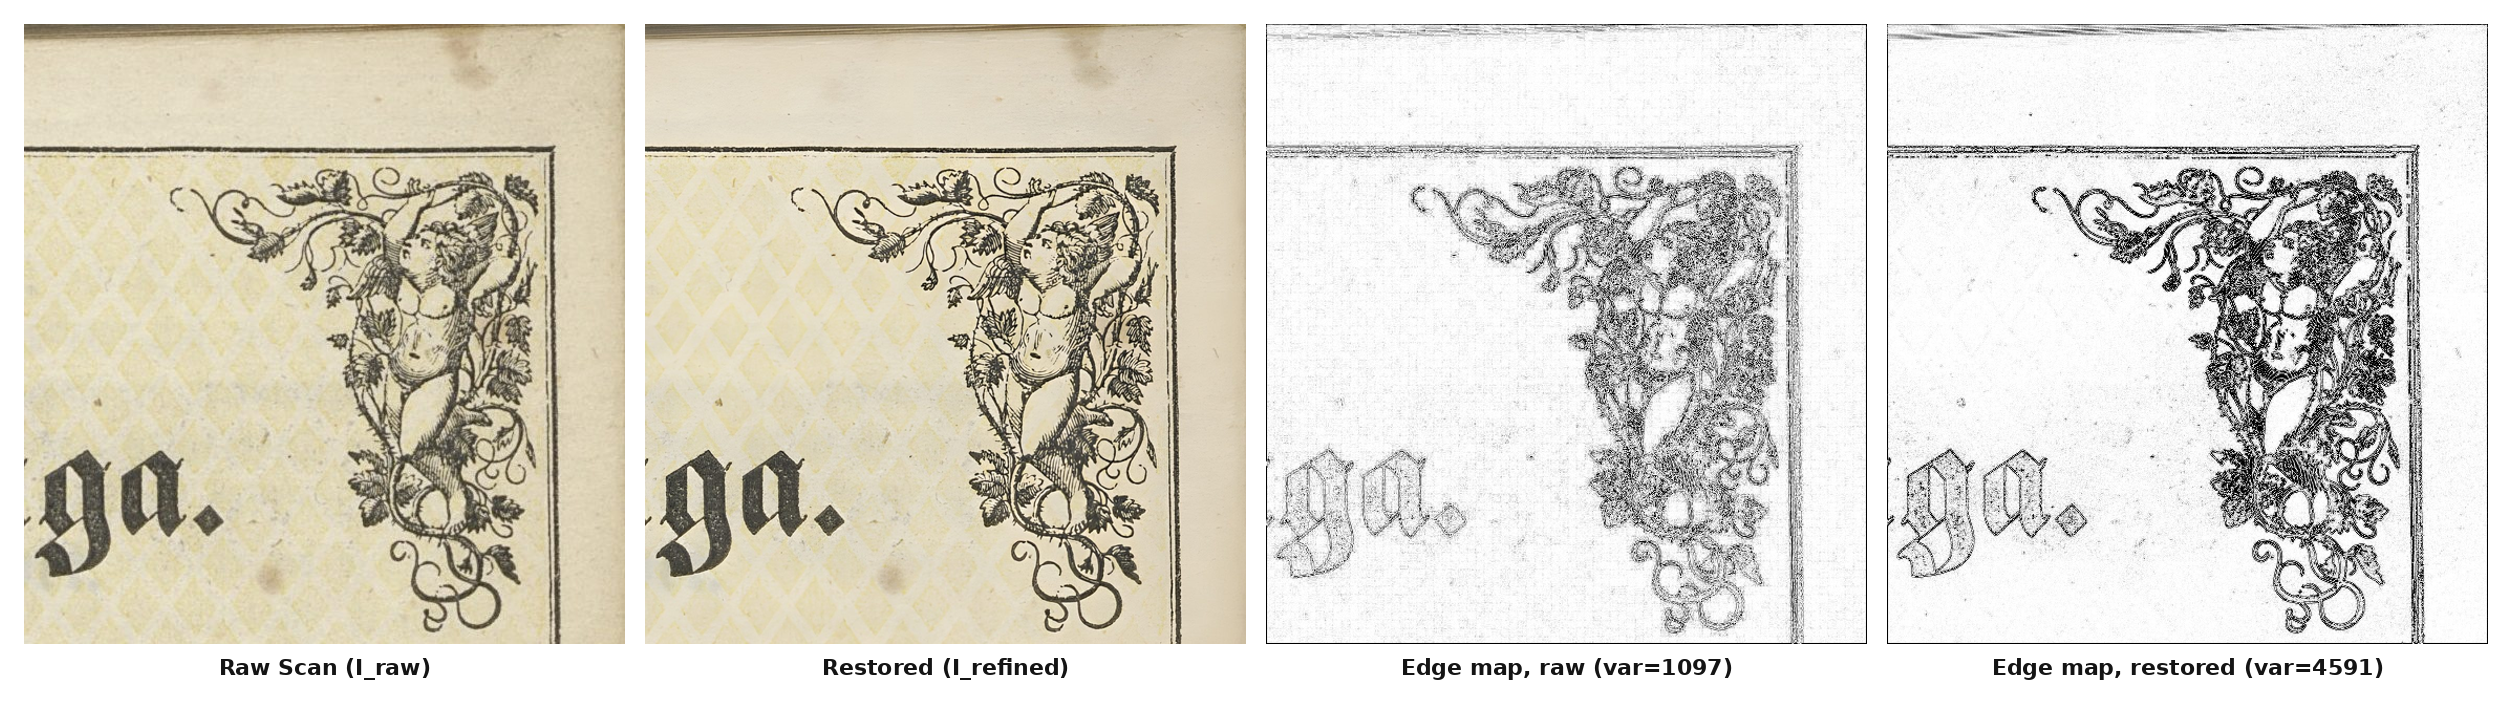
\includegraphics[width=\textwidth]{restoration_comparison_labeled.png}
\vskip 0.15cm
\footnotesize \textit{Raw scan / restored / Laplacian edge-response maps of the same crop. The pipeline is deliberately restrained (low diffusion strength, to avoid hallucinating content), so the difference is subtle to the eye at a glance -- the edge maps make it explicit: structural edge variance rises $1{,}097 \to 4{,}591$ (4.2$\times$) on this example, consistent with the $83.8\%$ population-level sharpness gain at left.}
\end{columns}
\end{frame}

\begin{frame}{A.2 AWLF v1 vs. AWLF v2 Error-Targeted Retraining}
\scriptsize
\scriptsize
\begin{columns}[T]
\column{0.50\textwidth}
\begin{alertblock}{AWLF v1: Scene-Presence Pathology}
\begin{itemize}
  \item AWLF v1 trained on binary \textit{scene presence}.
  \item Initial reference split contained extreme positive class imbalance ($319$ positive vs $2$ negative scans; $99.4\%$ positive rate).
  \item Trivial models achieved an inflated $\text{F1} = 0.9969$ simply by predicting all positive.
\end{itemize}
\end{alertblock}

\begin{block}{AWLF v2: Error-Targeted Retraining}
\begin{itemize}
  \item Target redefined strictly as classification failure: $y_i = \mathbb{I}[\operatorname{sign}(S_{\text{fusion},i}{\ge}0.5) \neq y_{\text{expert},i}]$.
  \item In-sample 5-fold CV on $C_1$: mean $\text{ROC-AUC} = 0.9897$ ($0.9896$ single fit).
  \item \textbf{Group-level held-out, corrected trustworthy pool} (Slide 3.5): $\text{ROC-AUC} = \mathbf{0.8702}$, vs $0.6669$ on the contaminated pool.
\end{itemize}
\end{block}


\column{0.46\textwidth}
\centering
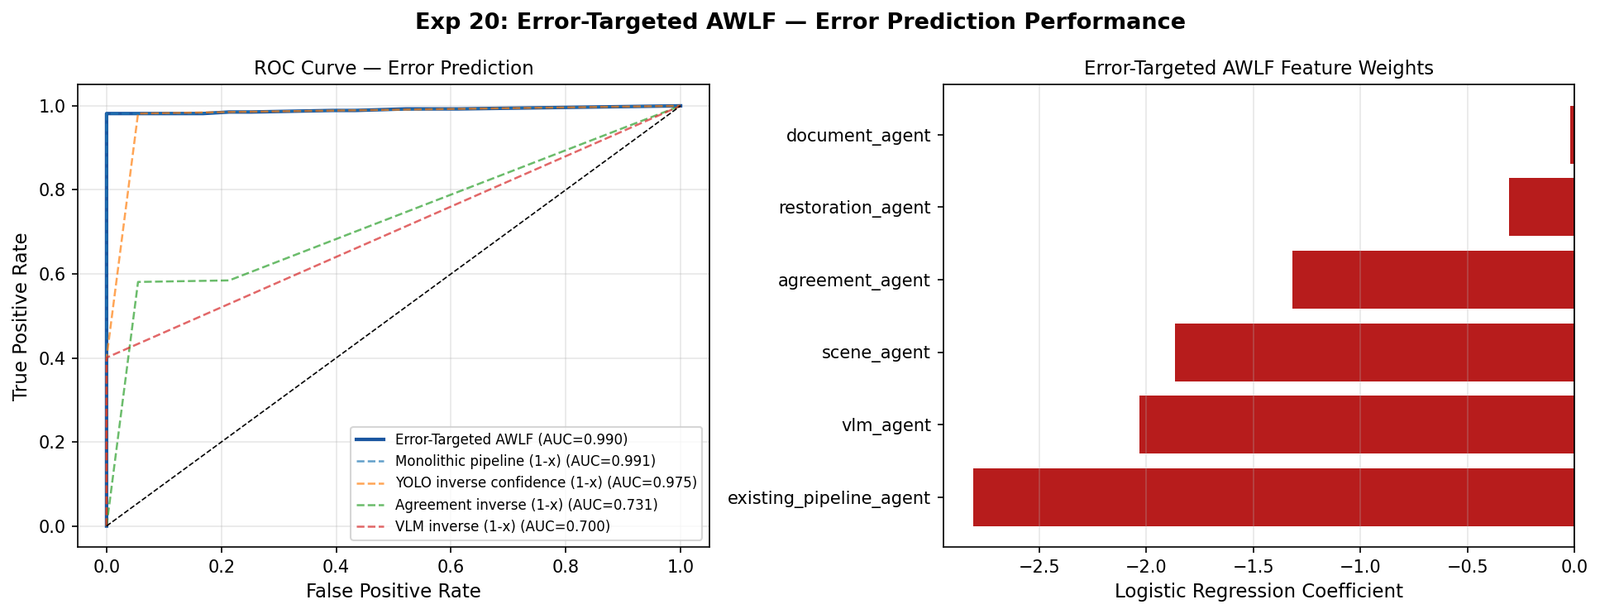
\includegraphics[width=0.92\textwidth]{exp20_error_awlf_roc_curve.png}
\vskip 0.1cm
\tiny \textit{AWLF v2 in-sample ROC ($C_1$; fit $0.9896$, 5-fold CV mean $0.9897$). Note the legend: the monolithic baseline scores marginally \emph{higher} in-sample ($0.991$ vs $0.990$) --- consistent with the thesis position that the strongest single-model baseline ties us on discrimination; the case rests on calibration and held-out behaviour. AWLF is a logistic model (gradient boosting scored $0.9857$).}
\end{columns}
\end{frame}

\begin{frame}{A.3 Semantic Ambiguity vs. Spatial Coordinate Disagreement}
\footnotesize
\begin{columns}[T]
\column{0.50\textwidth}
\begin{alertblock}{The Bounding-Box Error Paradox}
Using raw spatial detector confidence to detect human errors yields \evidence{$\text{ROC-AUC} = 0.4655$} (worse than random chance). Foundation detectors draw tight boxes with high confidence while misclassifying historical semantics.
\end{alertblock}

\begin{block}{Exp 31 Spatial Meta-Learner Resolution}
Training a Gradient-Boosted Meta-Learner on $C_2$ integrating box count, agent $\sigma$, mean confidence, $U_{\text{triage}}$ and the four agent scores resolves spatial layout ambiguity (\evidence{$\text{ROC-AUC} = 0.4655 \rightarrow \mathbf{0.6759 \pm 0.130}$}, 5-fold CV std).
\end{block}

\column{0.46\textwidth}
\centering
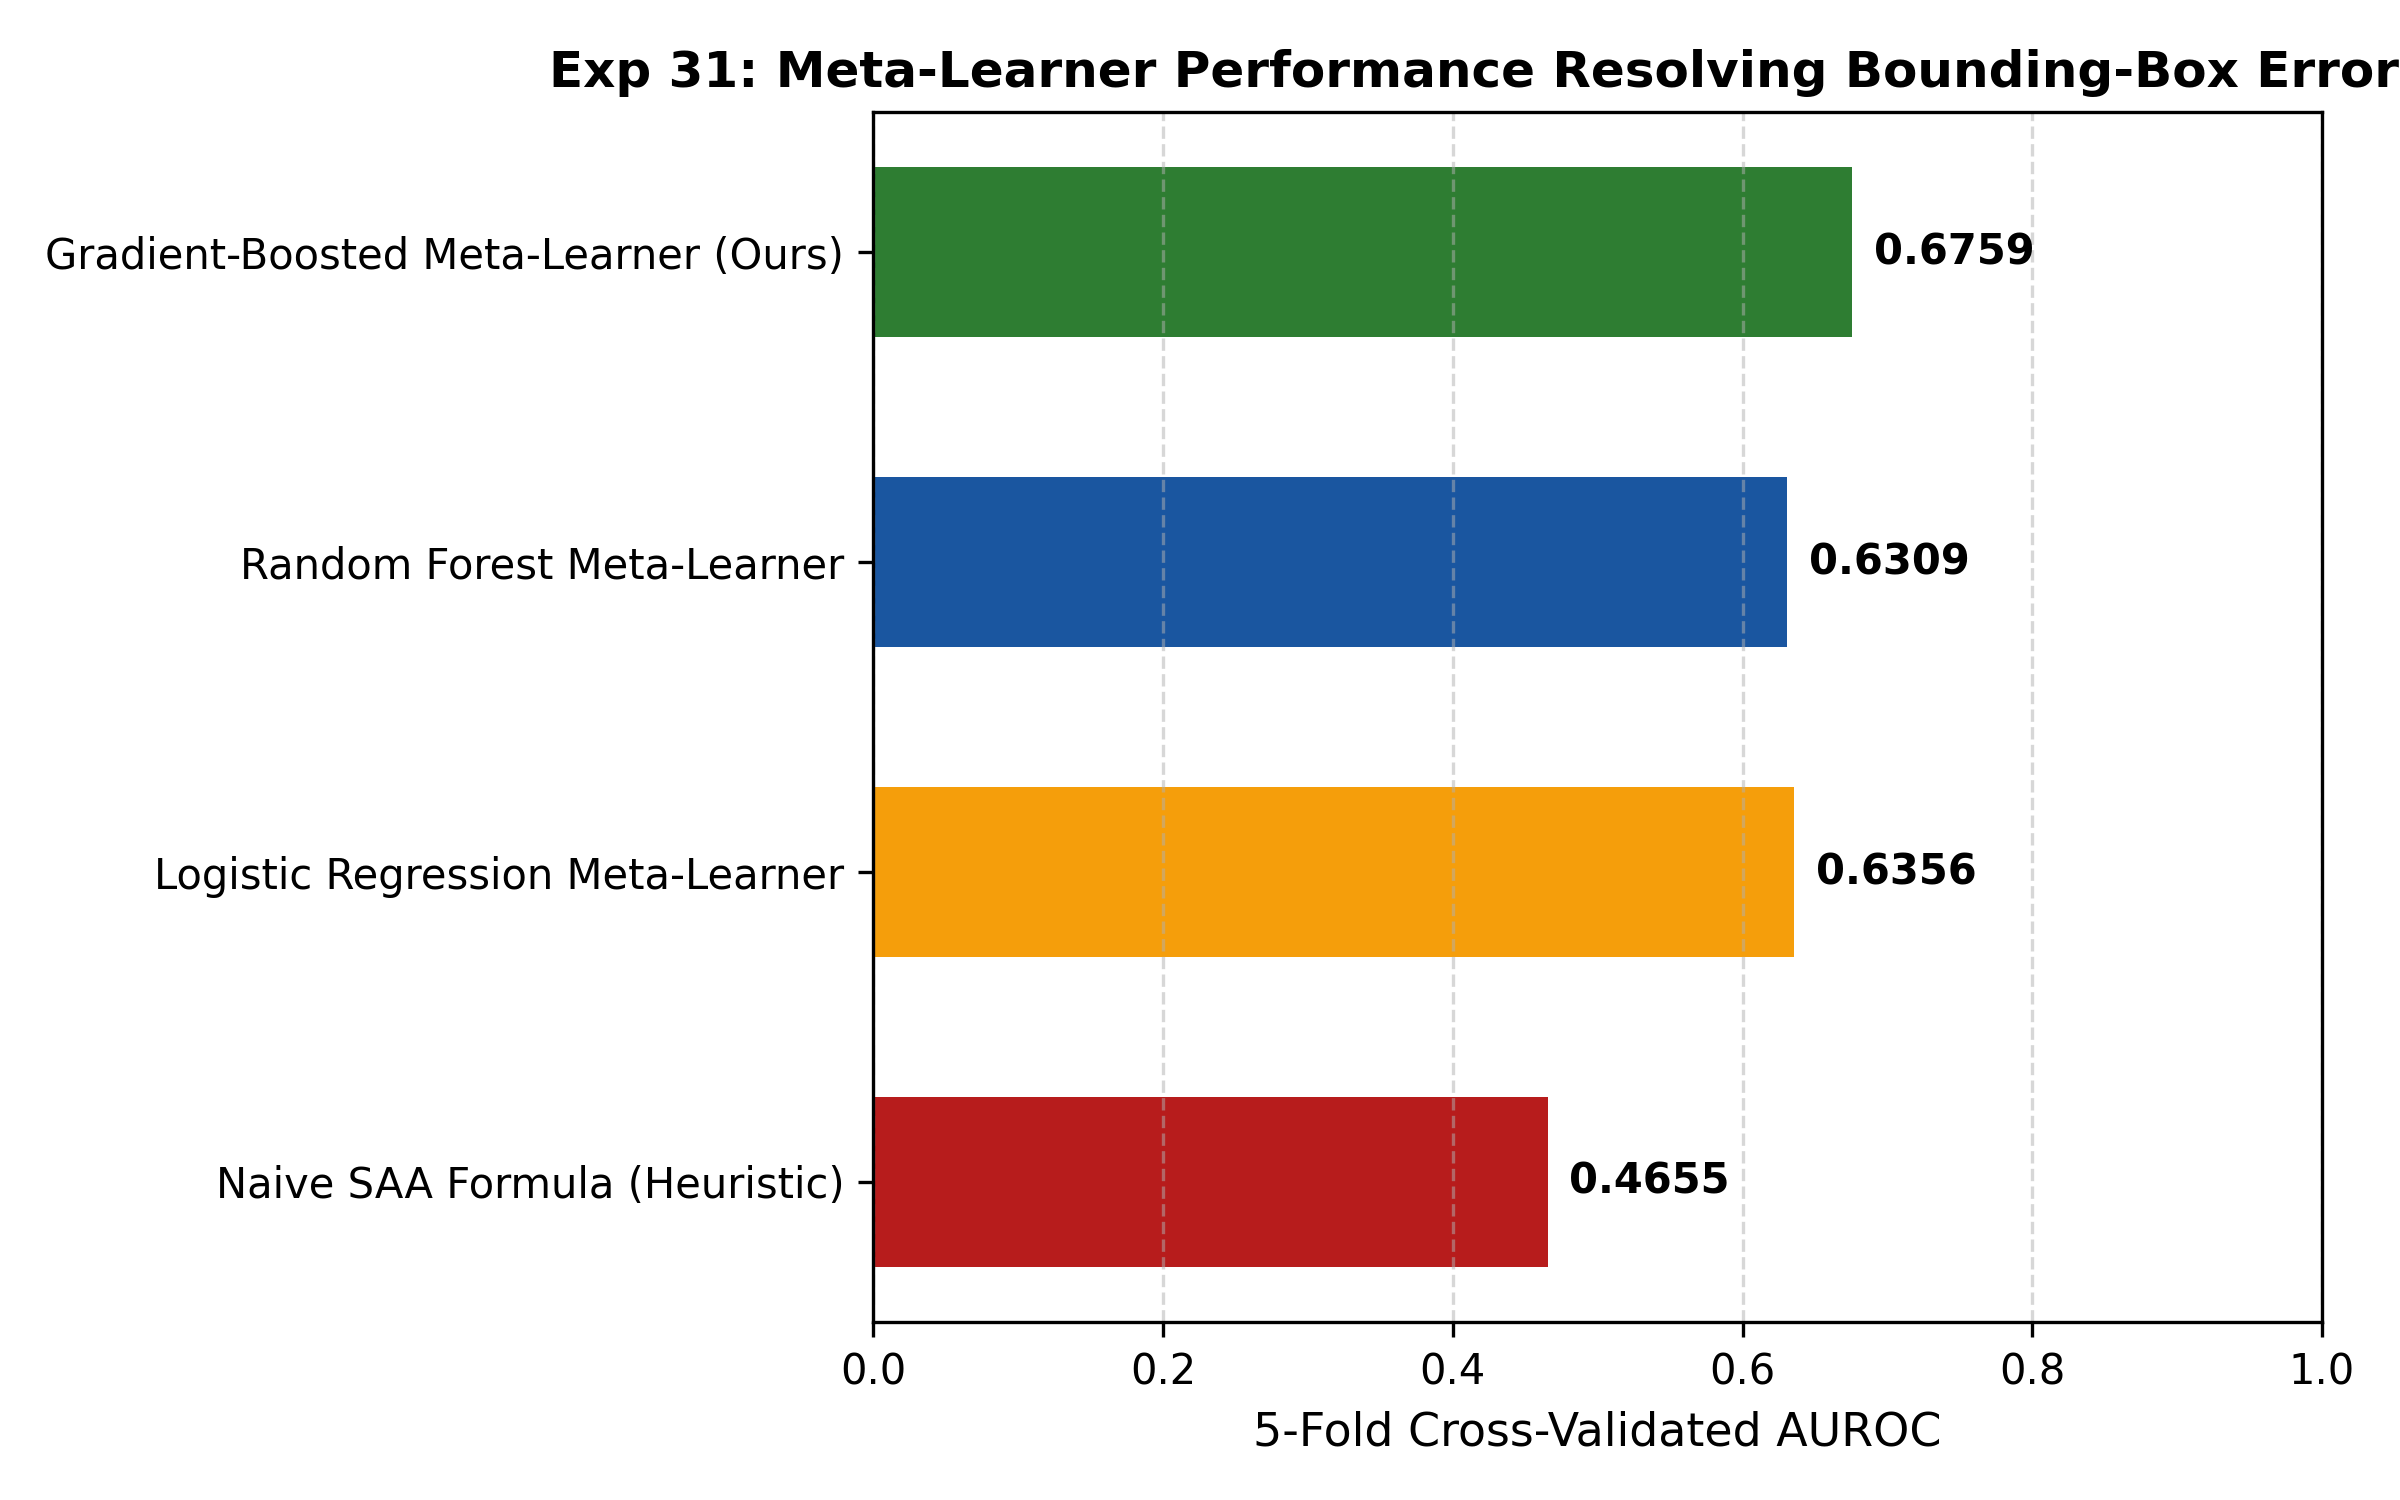
\includegraphics[width=\textwidth]{exp31_meta_learner_roc.png}
\vskip 0.1cm
\tiny \textit{5-fold cross-validated AUROC by meta-learner (Exp 31). Gradient boosting $0.6759$ vs logistic $0.6356$, random forest $0.6309$, naive SAA heuristic $0.4655$.}
\end{columns}
\end{frame}

\begin{frame}{A.4 Local Tier 3 Proxies: Same-Model Dropped, Disjoint-Model Retested}
\scriptsize
\begin{columns}[T]
\column{0.50\textwidth}
\begin{alertblock}{No Real Precision/Recall Comparison Exists}
\scriptsize A local-vs-frontier contradiction-detection F1 figure would require independently verified gold contradiction labels, which do not exist (Slide 2.3). Everything below is real inference, not a hardcoded number.
\end{alertblock}

\begin{block}{Step 1: Same-Model Critic Flag Rate}
\scriptsize Same Primary-then-Critic protocol:
\begin{itemize}
  \item \textbf{Local} (LLaVA-OneVision, $n=25$): \textbf{0/25} $\rightarrow$ dropped.
  \item \textbf{Stronger approx.} (Gemini Flash-Lite, $n=10$): \textbf{1/10}, still same-model.
\end{itemize}
Same weights just agree with themselves, regardless of capability.
\end{block}

\column{0.46\textwidth}
\begin{block}{Step 2: Genuinely Disjoint Local Models, Retested}
\scriptsize Two pairings, both directions -- both far above 0/25:
\begin{itemize}
  \item Qwen2.5-VL-72B $\leftrightarrow$ InternVL3.6-4B: \textbf{54\%}.
  \item Qwen2.5-VL-7B $\leftrightarrow$ LLaVA-7B (matched scale): \textbf{18\%}.
\end{itemize}
\end{block}
\begin{block}{What This Does and Doesn't Settle}
\scriptsize Visually verified: real catches exist, but so do real false alarms (one critic invented a claim, then flagged its own invention). Disjoint weights catch what same weights can't -- but the flag rate isn't trustworthy precision alone. Deployed pair (Gemini/Claude) still untested.
\end{block}
\end{columns}
\end{frame}

\begin{frame}{A.5 External Cross-Depiction Benchmark: PeopleArt ($n=4,778$)}
\footnotesize
\begin{columns}[T]
\column{0.52\textwidth}
\begin{block}{Cross-Style Generalization ($n=4,778$ Images, 43 Styles)}
\scriptsize
\resizebox{\linewidth}{!}{%
\begin{tabular}{lccc}
\toprule
\textbf{Style Category} & \textbf{Precision} & \textbf{Recall} & \textbf{F1-Score} \\
\midrule
Photo & 0.875 & 0.915 & \textbf{0.878} \\
Realism & 0.840 & 0.874 & 0.835 \\
Impressionism & 0.888 & 0.944 & 0.880 \\
Cubism & 0.836 & 0.834 & 0.831 \\
Cartoon & 0.706 & 0.680 & 0.673 \\
\bottomrule
\end{tabular}%
}
\end{block}

\begin{block}{Key Generalization Finding}
\scriptsize
Real YOLO detection degrades gracefully as style diverges from photorealism, to Cartoon ($F_1=0.673$).
\end{block}

\column{0.44\textwidth}
\centering
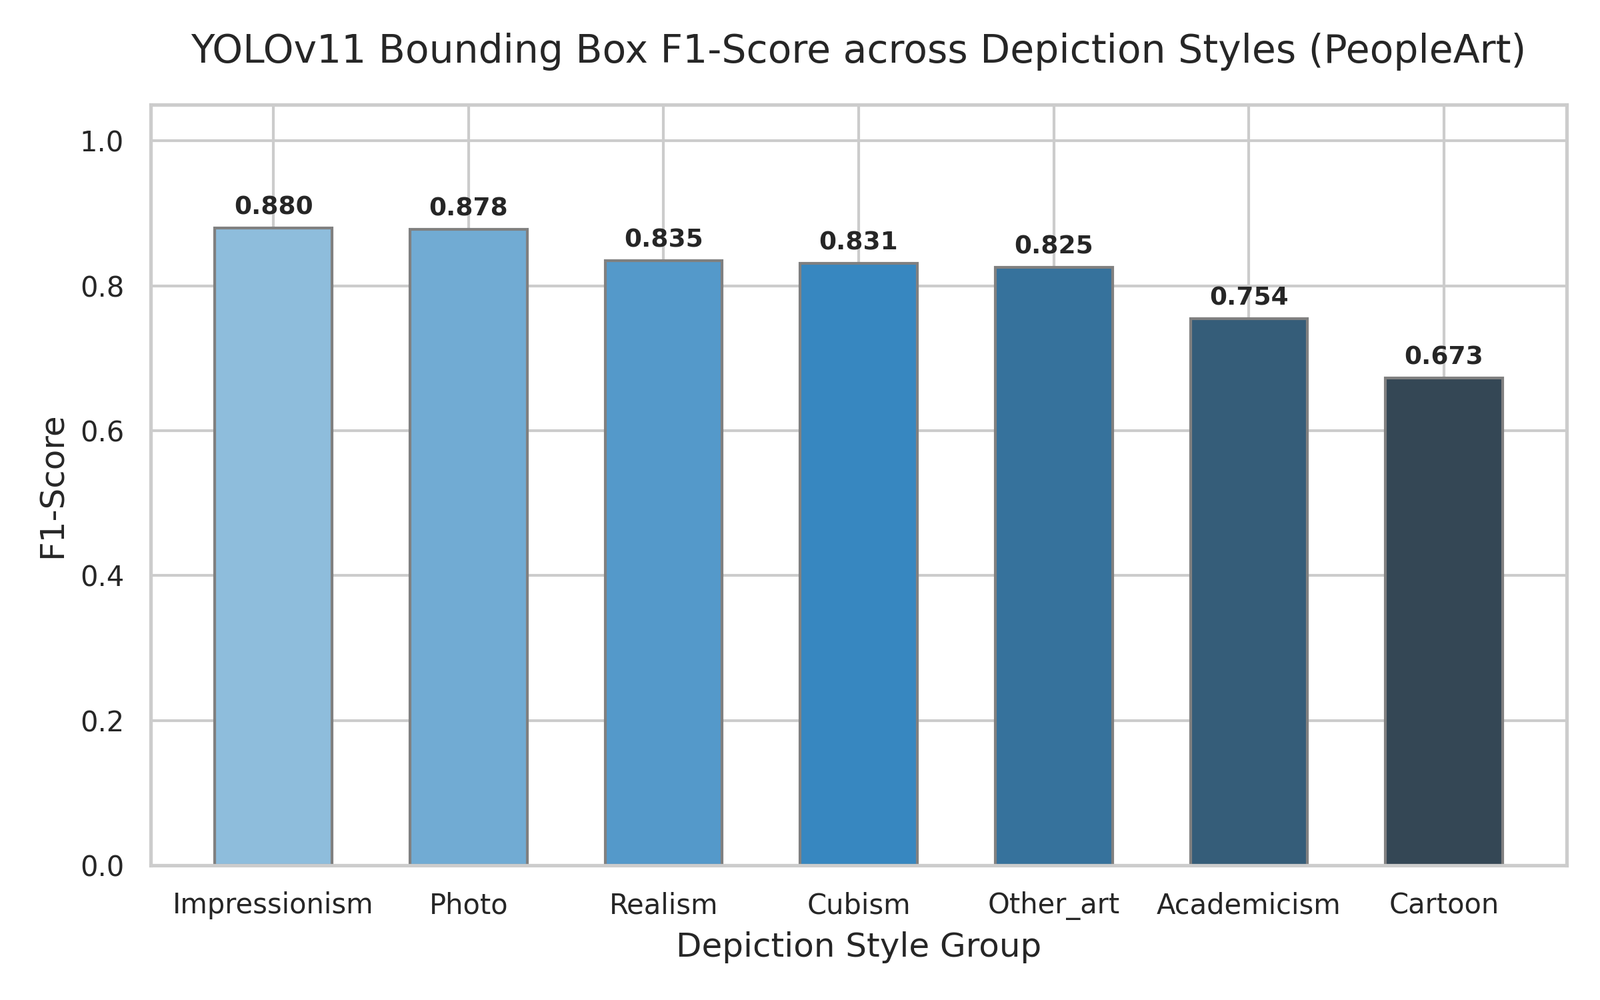
\includegraphics[width=\textwidth]{peopleart_style_f1.png}
\vskip 0.1cm
\tiny \textit{PeopleArt F1-Score by Style (real YOLO detections vs.\ ground truth).}
\end{columns}
\end{frame}

\begin{frame}{A.6 Cross-Institutional Europeana Transfer Pilot ($C_5, n=24$)}
\scriptsize
\begin{columns}[T]
\column{0.50\textwidth}
\begin{block}{Genuine Europeana API Pilot}
\begin{itemize}
    \item 24 images live-downloaded, 10 verified GLAM institutions; all 4 Tier 1 signals really measured.
    \item SAA fusion \textbf{0.332} vs.\ Colibri's \textbf{0.764} -- a real domain-shift response.
    \item Now labelled (23 of 24): all scene-positive, and the unchanged pipeline \textbf{misses 15} ($65.2\%$). YOLO found nothing on 12.
\end{itemize}
\end{block}

\begin{alertblock}{Why the Signal Can't Be Scored Here}
The ensemble collapsed: \textbf{effective rank 1.37} of 4 (CI 1.06--1.61) vs \textbf{2.50} on Colibri -- the VLM contributes std $0.051$ instead of $0.320$. With ~1 independent direction left, ``disagreement'' restates one number. \textbf{A checkable precondition}, needing no labels (A.13).
\end{alertblock}

\column{0.44\textwidth}
\centering
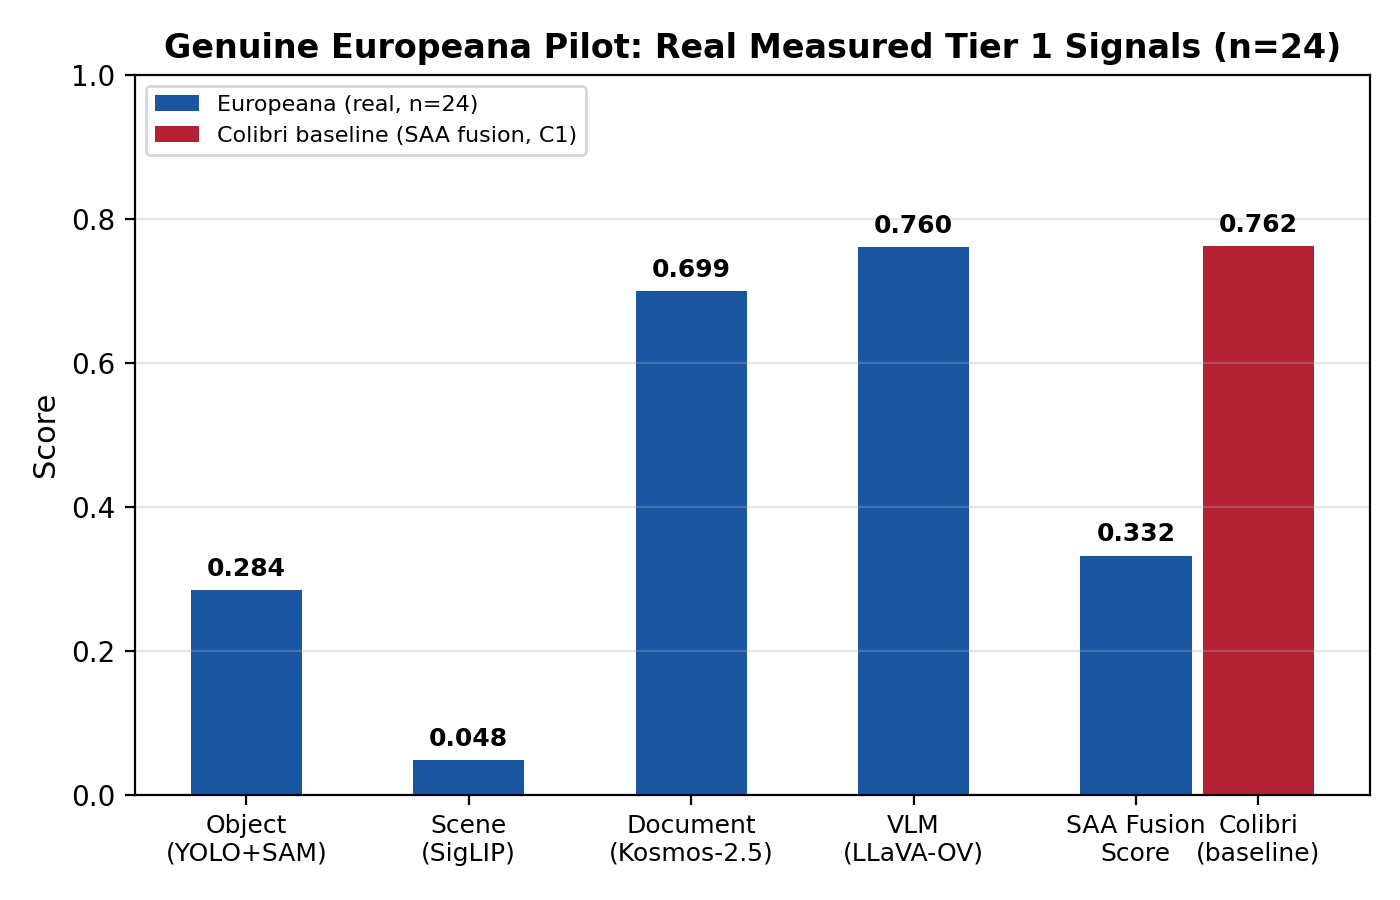
\includegraphics[width=\textwidth]{europeana_real_pilot_signals.png}
\vskip 0.1cm
\tiny \textit{Real measured Tier 1 signals on genuine Europeana images ($n=24$) vs.\ Colibri baseline.}
\end{columns}
\end{frame}

\begin{frame}{A.7 Hardware Resource Consumption \& Inference Latency}
\tiny
\centering
\textit{Deployment reference figures, not a methodological contribution -- informal single-image timings rather than a controlled benchmark. A YOLOv11 spot-check found raw forward-pass time near the table's $0.02$s, but end-to-end latency (incl.\ I/O, pre/post-processing) measured $3$--$8\times$ higher; other rows not independently re-measured.}
\vskip 0.2cm
\begin{table}[!htbp]
\caption{Hardware Resource Consumption and Per-Stage Latency (NVIDIA RTX A6000 48GB).}
\begin{tabular}{lrr}
\toprule
\textbf{Pipeline Stage / Model Backbone} & \textbf{VRAM Consumption} & \textbf{Latency / Image} \\
\midrule
CycleGAN Domain Translation & 4.2 GB & 0.15s \\
Real-ESRGAN $4\times$ Upscaling & 8.5 GB & 0.45s \\
Stable Diffusion Img2Img Refinement & 12.1 GB & 3.20s \\
Florence-2 Grounded Detection & 18.0 GB & 1.20s \\
GroundingDINO Object Detection & 22.4 GB & 2.10s \\
LLaVA-OneVision 7B VQA Reasoning & 34.2 GB & \textbf{1.56s} \\
\textbf{YOLOv11 Distilled Local Inference} & \textbf{1.8 GB} & \textbf{0.06s} \\
\bottomrule
\end{tabular}
\end{table}

\begin{block}{Deployability Highlight}
The distilled student detector runs at \textbf{0.06s/image}, measured end to end over all $12{,}110$ images ($\approx25\times$ faster than LLaVA-OneVision 7B), enabling real-time deployment on institutional archive servers.
\end{block}
\end{frame}

\begin{frame}{A.8 Reproducibility, and Real Inter-Annotator Agreement}
\scriptsize
\begin{block}{Every Cited Number Regenerates From One Command}
\texttt{bash scratch/run\_full\_master\_experiments.sh} --- 42 steps, about a minute, \textbf{no GPU and no paid API calls}. Last full verification:
\begin{itemize}\scriptsize
  \item \textbf{159 of 161} result artifacts reproduced \emph{byte-identically}. The two exceptions differ only in the final floating-point digit and are cited nowhere.
  \item \textbf{17 of 17} cited headline figures matched the freshly regenerated artifacts exactly (SAA $0.860$, AWLF $0.8702$, $0.9687$/$0.1259$, CRC $0.0201$/$60.6\%$/$91.1\%$/$2.31\times$, Agent 2/4/5, Europeana).
  \item Key scripts carry a \texttt{-{}-verify} flag that recomputes and \emph{fails loudly} if an artifact has drifted.
  \item \texttt{REPRODUCE.md} maps every claim to the script and artifact that produce it.
\end{itemize}
\end{block}

\begin{block}{Real Inter-Annotator Agreement (124 of 300 $C_1$/$C_2$ Images)}
\scriptsize Only 124 of $C_2$'s 300 images land in $C_1$'s genuinely reviewed range; the other 176 matched an unverified default-labelled portion of the pool and are \emph{excluded}, not counted as a second rater. On those 124: categorical Cohen's $\kappa=\mathbf{0.337}$, raw agreement $\mathbf{83.9\%}$ --- ``fair'' (Landis \& Koch). Binary has-scene $\kappa$ is undefined here: all 5 of $C_1$'s real negatives fall outside this overlap, so Rater A has zero variance on that axis.
\end{block}
\end{frame}

\begin{frame}{A.9 Game-Theoretic Shapley Attribution (Backup)}
\footnotesize
\begin{columns}[T]
\column{0.50\textwidth}
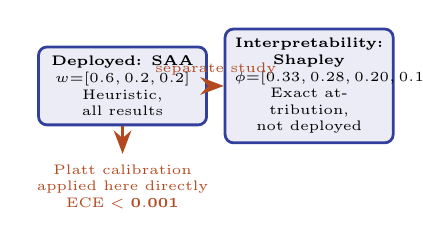
\begin{tikzpicture}[
  node distance=0.25cm and 0.2cm,
  every node/.style={font=\tiny},
  stagebox/.style={draw=HildesheimRed, fill=PrismRed!10, rounded corners=3pt, align=center, text width=1.9cm, minimum height=0.9cm, line width=1pt},
  arrow/.style={->, >=Stealth, line width=1.2pt, PrismOrange}
]
\node[stagebox] (s1) {\textbf{Deployed: SAA}\\$w{=}[0.6,0.2,0.2]$\\Heuristic, all results};
\node[stagebox, right=of s1] (s2) {\textbf{Interpretability: Shapley}\\$\phi{=}[0.33,0.28,0.20,0.19]$\\Exact attribution, not deployed};

\draw[arrow, dashed] (s1) -- (s2) node[midway, above, font=\tiny] {separate study};
\draw[arrow] (s1.south) -- ++(0,-0.35) node[below, font=\tiny, align=center] {Platt calibration\\applied here directly\\$\mathbf{\text{ECE} < 0.001}$};
\end{tikzpicture}

\vskip 0.2cm
\begin{block}{Exp 30 Shapley Attribution Results}
LLaVA-OneVision 7B ($\phi_1 = 0.330, 33.0\%$) and SAA Core ($\phi_2 = 0.283, 28.3\%$) provide over $61\%$ of total diagnostic signal.
\end{block}
\begin{alertblock}{\scriptsize Not the Deployed Weighting}
\scriptsize A supplementary interpretability study only -- quantifies contribution to a coalitional objective, not independent causal correctness. No result elsewhere uses these Shapley weights.
\end{alertblock}

\column{0.46\textwidth}
\centering
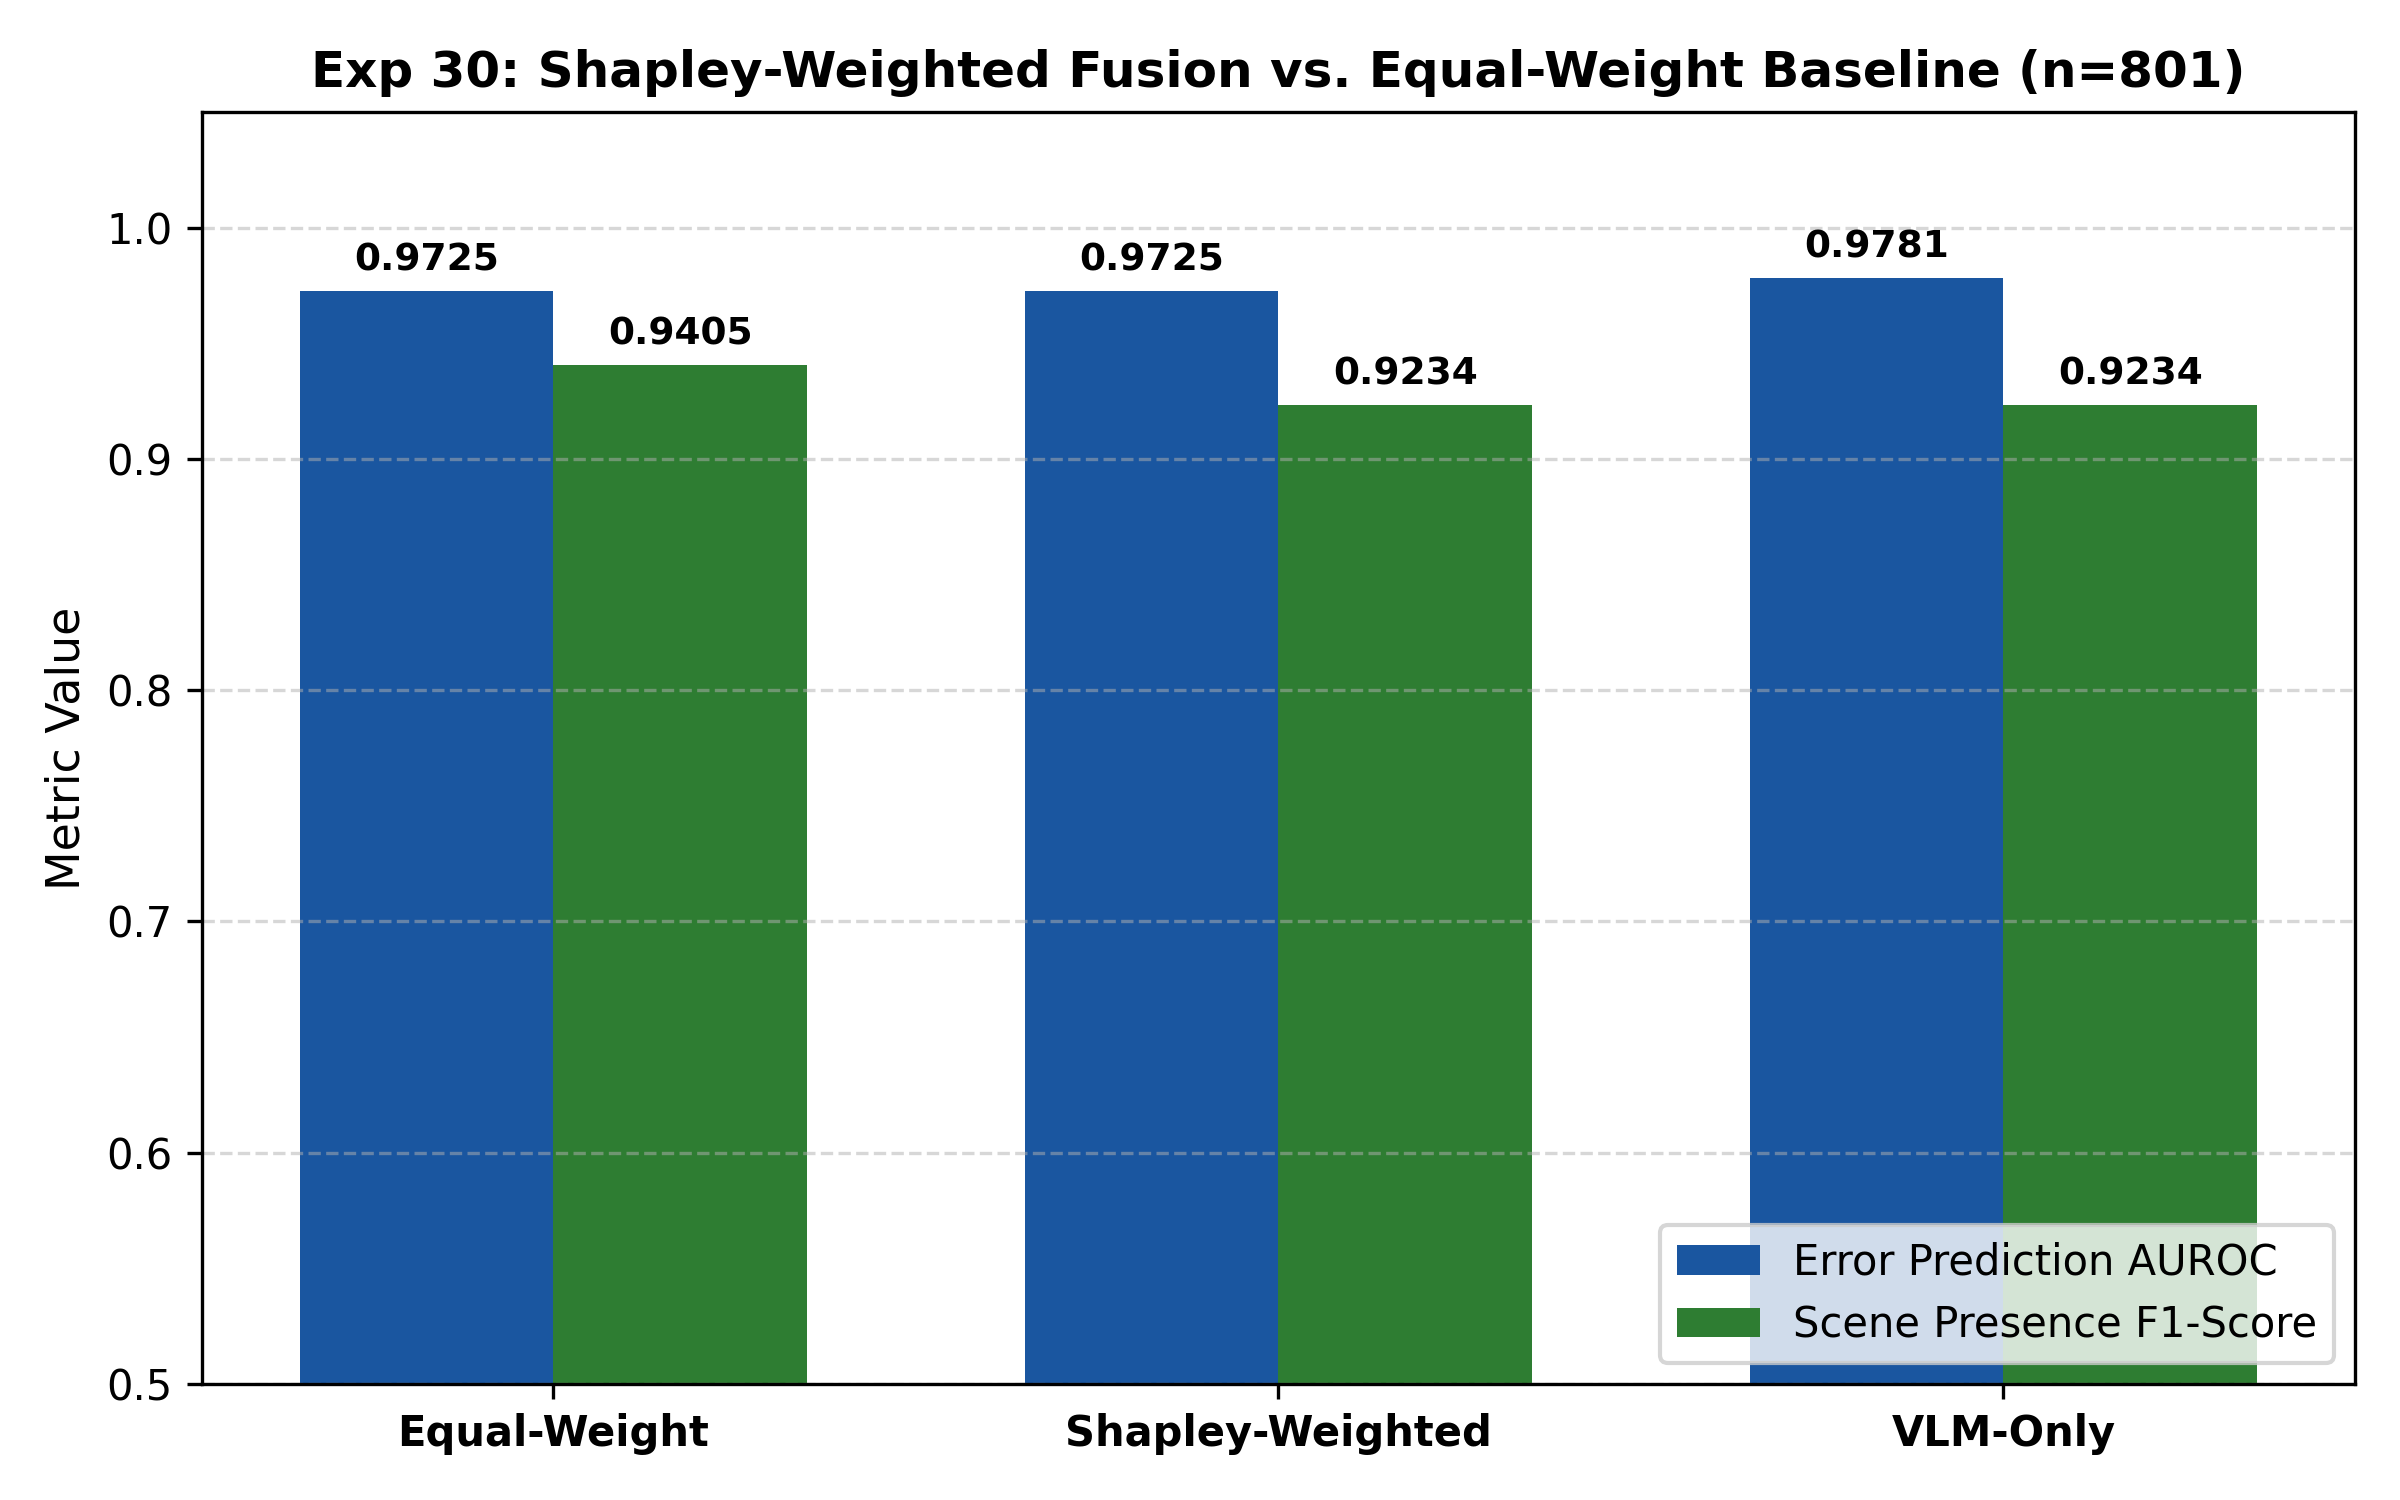
\includegraphics[width=\textwidth]{exp30_shapley_fusion_bars.png}
\vskip 0.1cm
\tiny \textit{Downstream performance of Shapley-weighted fusion vs.\ equal-weight and VLM-only -- not a plot of the $\phi_i$ values themselves (those are at left).}
\end{columns}
\end{frame}

\begin{frame}{A.10 Agents 2 \& 5: Real Gold-Labeled Benchmarks (Backup Detail)}
\scriptsize
\begin{columns}[T]
\column{0.5\textwidth}
\begin{block}{Agent 2: Real Signal, Imprecise Framing}
$101$ gold-labeled candidates (all $25$ disagreement images): $21$ genuine hallucinations, $69$ YOLO misses, $11$ ambiguous $\to$ \textbf{$23.3\%$ precision} as a hallucination detector. Qualitative pattern confirmed in 3 detailed cases: 2 clean YOLO misses (VLM correctly says ``dog''/``animal'', YOLO says \{sack\}); 1 complex case where VLM is mostly \emph{right} and YOLO misses horse/building/trees. Diagnosis: usually \textbf{YOLO under-detection}, not VLM hallucination.
\end{block}
\begin{alertblock}{Two Real Noise Sources}
\scriptsize VLM occasionally echoes the entire prompt category list (spurious flags); free-text nouns need synonym normalization vs.\ YOLO's fixed vocabulary.
\end{alertblock}

\column{0.5\textwidth}
\begin{block}{Agent 5: Real 3-Bucket Corpus Benchmark}
corpus-wide, all $n=12{,}110$: $\mathbf{49.8\%}$ degenerate repetition, $\mathbf{\ge 3.4\%}$ hallucinated captioning (pattern-matched), $\mathbf{46.4\%}$ candidate real OCR.
\end{block}
\begin{block}{Confirmed at Scale: 53 Gold-Labeled Images}
Classifier validated on only 1 of 3 buckets: hallucinated captioning $\mathbf{100\%}$ correct (5/5); degenerate repetition only $\mathbf{50\%}$ (4/8 actually have real text Kosmos missed); candidate real OCR only $\mathbf{52.5\%}$ (21/40 actually have text) -- median WER $100\%$ even then.
\end{block}
\end{columns}
\vskip 0.15cm
{\tiny\color{PrismGray} Both agents now have real, gold-labeled population-level precision figures ($n=101$, $n=53$) -- not single-rater spot-checks.}
\end{frame}

\begin{frame}{A.11 Agent 4: Underlying Data-Quality Check (Backup Detail)}
\scriptsize
Agent 4 embeds VLM scene descriptions to find cross-PPN nearest neighbors. Corpus-wide check (all $n=12{,}110$) of the raw material those embeddings are built from:
\begin{columns}[T]
\column{0.5\textwidth}
\begin{alertblock}{Pipeline Bug: Errors Stored as Content}
$8$ records ($0.07\%$) contain a literal \texttt{HTTPConnectionPool... Read timed out} string in place of real VLM output -- would silently corrupt any embedding built from it.
\end{alertblock}

\column{0.5\textwidth}
\begin{alertblock}{Cross-Lingual Hallucination}
$\mathbf{2{,}325}$ records ($\mathbf{19.2\%}$) contain injected Chinese-character tokens inside German/English output (e.g.\ ``\ldots der\,[U+5F1B][U+63A3]\,Er'') -- on a corpus with no Chinese source material.
\end{alertblock}
\end{columns}
\begin{block}{Practical Consequence (TF-IDF Proxy, Not the Deployed Method)}
Among the highest-similarity cross-PPN description pairs (sampled $n=2{,}996$), several score a perfect $1.000$ purely because both records share the same stored error string or hallucination pattern -- not real compositional similarity. Agent 4's real embedding method may not reproduce these exact false matches, but its raw input material is measurably unreliable for a meaningful fraction of the corpus.
\end{block}
{\tiny\color{PrismGray} Corpus-wide mechanical check of the upstream text material Agent 4's embeddings are built from -- see A.12 for a real benchmark of the mechanism itself.}
\end{frame}

\begin{frame}{A.12 Agent 4: Real Visual-Embedding Benchmark (Backup Detail)}
\scriptsize
Genuine SigLIP image embeddings (same model family as Agent 3) for $400$ accessible images, ranked by cosine similarity over cross-PPN pairs only -- much closer to Agent 4's real mechanism than the text proxy (A.11).
\begin{columns}[T]
\column{0.5\textwidth}
\begin{block}{A Genuine Match (sim $=0.938$)}
The single highest-similarity pair is the literal \emph{same illustration} reprinted across two different digitized volumes -- identical figures and composition, visually confirmed. The mechanism works when a real match exists.
\end{block}

\column{0.5\textwidth}
\begin{alertblock}{A Real Limitation (sim $=0.901$)}
The next-highest pair is visually confirmed to be two \emph{different} compositions (a court scene, a street scene) sharing only engraving style and period costume -- not the same picture.
\end{alertblock}
\end{columns}
\begin{block}{Confirmed at Scale: 79 Gold-Labeled Pairs}
Overall precision $\mathbf{55.7\%}$ ($44$ genuine / $30$ style-only / $5$ unrelated), rising monotonically and reaching a stable $\mathbf{100\%}$ plateau at similarity $\ge 0.92$ ($n=41$). \textbf{Deployment recommendation}: threshold at $\ge 0.92$.
\end{block}
{\tiny\color{PrismGray} A real, gold-labeled population-level precision-at-threshold curve ($n=79$) -- not just the two-pair spot-check above.}
\end{frame}

\begin{frame}{A.13 The Heterogeneity Precondition (Backup Detail)}
\scriptsize
Before applying a disagreement method to a new archive, one thing is checkable \emph{without labels}: does the ensemble still span enough independent directions for ``disagreement'' to mean anything? Effective rank $=\exp(-\sum_i p_i \log p_i)$ over the normalised agent-covariance eigenvalues answers it.

\begin{center}\scriptsize
\begin{tabular}{lccc}
\toprule
\textbf{Cohort} & \textbf{$n$} & \textbf{Eff.\ rank (4 signals)} & \textbf{Eff.\ rank (3 genuine)} \\
\midrule
Colibri $C_0$ & $12{,}110$ & $2.50$ {\tiny[2.48, 2.51]} & $2.17$ {\tiny[2.15, 2.19]} \\
Europeana $C_5$ & $24$ & $\mathbf{1.37}$ {\tiny[1.06, 1.61]} & $\mathbf{1.50}$ {\tiny[1.06, 1.79]} \\
\bottomrule
\end{tabular}
\end{center}

\begin{block}{\scriptsize Why the Intuitive Diagnostics Mislead}
\tiny All three plausible symptoms fail a control -- each holds just as strongly on Colibri, where the method works. The VLM takes two distinct values (true on \emph{both}); fusion correlates with one agent ($r=0.993$ vs $0.980$ -- the $0.6$ object weight makes it object-dominated everywhere); the scene agent looks flat (Europeana has \emph{more} distinct values, $22$ vs $2$). \textbf{Discreteness is not degeneracy.}
\end{block}

\begin{alertblock}{\scriptsize The Practical Point}
\tiny Run it first, on scores alone, before spending annotation budget. Below $2$, a disagreement score restates one number and its ROC-AUC is an artifact. The $2.0$ threshold separates the regimes under \emph{both} parameterisations with disjoint CIs -- so this does not depend on the derived Agreement term (A.14).
\end{alertblock}
\end{frame}

\begin{frame}{A.14 What Is $U_{\text{SAA}}$ Actually Measuring? (Backup Detail)}
\footnotesize
\scriptsize $U_{\text{SAA}}=\operatorname{std}(A^{\text{obj}}, A^{\text{agree}}, A^{\text{scene}}, A^{\text{vlm}})$, but $A^{\text{agree}}=1-|A^{\text{obj}}-A^{\text{vlm}}|$, and $A^{\text{vlm}}=\mathbb{I}[A^{\text{obj}}>0]$ on \emph{all} $12{,}110$ images. Three of four terms are functions of $A^{\text{obj}}$ alone, so $U_{\text{SAA}}$ takes exactly \textbf{8 distinct values} corpus-wide.
\vskip 2pt
\scriptsize \textbf{Why.} Not model agreement --- two of the four signals turned out to share one source. A.18.

\vspace{-3.5mm}
\begin{block}{\scriptsize The structural consequence}
\tiny When Object and VLM agree at \emph{low} values the derived term jumps to $1$ and inflates the spread: unanimous-absent $(0,0)\rightarrow\mathbf{0.479}$ vs unanimous-present $(1,1)\rightarrow 0.250$. Maximal uncertainty where the ensemble is unanimous, if the verdict is negative.
\end{block}

\vspace{-3mm}
\begin{center}\scriptsize
\begin{tabular}{lcc}
\toprule
\textbf{Uncertainty signal} & \textbf{$C_1$ ($n{=}801$)} & \textbf{Held-out ($n{=}249$)} \\
\midrule
$U_{\text{SAA}}$ as deployed (incl.\ derived term) & $\mathbf{0.9724}$ & $\mathbf{0.8600}$ \\
$1 - A^{\text{object}}$ (single-model confidence) & $0.9726$ & $0.8722$ \\
$1 - \bar{A}$, 3 genuine agents (pure confidence) & $0.9717$ & $0.8799$ \\
$\sigma$ over 3 genuine agents (derived removed) & $0.7694$ & $0.8340$ \\
\bottomrule
\end{tabular}
\end{center}

\vspace{-3mm}

\begin{alertblock}{\scriptsize What I claim, and what I don't}
\tiny Top three rows are statistically tied, and CRC certifies risk relative to whatever score it is given, so the guarantee is unaffected. What I do \textbf{not} claim is that \emph{disagreement} detects the errors --- and rebuilt from raw outputs, retested without the circularity, that still holds (A.18).
\end{alertblock}
\end{frame}

\begin{frame}{A.15 Two Error Labels in the Pipeline (Backup Detail)}
\footnotesize
\scriptsize The thesis defines $SAA_i = 0.6A^{\text{obj}} + 0.2A^{\text{scene}} + 0.2A^{\text{vlm}}$ and previously said this was used for every result. \textbf{That was not accurate}; the correction is reported rather than quietly reconciled.

\begin{block}{\scriptsize What is actually deployed}
\tiny \texttt{comparison\_fusion\_score} fixes the label for the in-sample $C_1$ result and \emph{all} CRC experiments. No script recomputes it; least squares recovers it exactly (max dev $3.1\times10^{-7}$) as $\tfrac{1}{3}A^{\text{obj}} + \tfrac{4}{15}A^{\text{agree}} + \tfrac{1}{5}A^{\text{scene}} + \tfrac{1}{5}A^{\text{vlm}}$ -- a \textbf{four}-agent fusion carrying the derived Agreement term at $0.267$. The labels disagree on $22.1\%$ of the pool, and since the deployed label contains $A^{\text{agree}}$, label and predictor share it -- tightening A.14's circularity.
\end{block}

\begin{center}\scriptsize
\begin{tabular}{lcc}
\toprule
 & \textbf{deployed label} & \textbf{thesis's stated label} \\
\midrule
$\hat\lambda$ / risk / approval & $0.372$ / $0.0201$ / $60.64\%$ & $0.372$ / $0.0201$ / $60.64\%$ \\
error recall & $91.07\%$ & $92.86\%$ \\
efficiency lift & $2.31\times$ & $2.36\times$ \\
\midrule
in-sample ROC-AUC & $\mathbf{0.9724}$ & $\mathbf{0.9586}$ \\
\bottomrule
\end{tabular}
\end{center}

\vskip 0.1cm
\begin{alertblock}{\scriptsize What Moves and What Does Not}
\tiny \textbf{Every CRC number stands under either convention} -- threshold, risk and approval are identical, bound holds both ways, and recall/lift shift favourably. The in-sample figure is the sensitive one, now reported as label-specific.
\end{alertblock}
\end{frame}

\begin{frame}{A.16 Probing the Stated Limitations (Backup Detail)}
\scriptsize
Of the six limitations this thesis states, four are empirically decidable. All figures below are fitted on the training
partition and scored on the held-out test split ($n=249$, $70$ errors).
\vspace{1mm}
\begin{center}
\tiny
\begin{tabular}{@{}p{2.3cm}p{3.7cm}p{4.6cm}@{}}
\toprule
\textbf{Limitation} & \textbf{What was run} & \textbf{Result} \\
\midrule
Single model does as well & All four agents \emph{plus} the two measured signals no level uses, vs.\ one agent & $0.8703$ vs $0.8722$; $\Delta=-0.002$, CI $[-0.043,0.038]$. \textbf{Confirmed} --- the extra signals do not rescue it \\
\addlinespace
Disagreement is not what works & Confidence alone vs.\ confidence $+\ U_{\text{SAA}}$ & $0.8799$ vs $0.8810$; $\Delta=+0.001$, CI $[-0.000,0.004]$. \textbf{Confirmed}, now out of sample \\
\addlinespace
Fails on no-scene images & Train a gate to flag no-scene, abstain on what it flags & Gate reaches AUROC $\mathbf{0.798}$; abstaining on $10\%$ gains $+0.013$, CI $[-0.014,0.040]$. \textbf{Predictable, not repairable} \\
\addlinespace
Not causal & Remove one agent at a time --- an intervention, not an attribution & VLM: $0.86\to0.72$, CI $[-0.195,-0.098]$, \textbf{excludes zero}. Object: \textbf{exactly} $0.000$ \\
\bottomrule
\end{tabular}
\end{center}
\end{frame}

\begin{frame}{A.17 Reading the Limitation Probes (Backup Detail)}
\footnotesize
\begin{itemize}
  \setlength\itemsep{3pt}
  \item \textbf{Why removing the object agent changes nothing.} It maps the eight distinct $U_{\text{SAA}}$ values through a strictly increasing bijection (Spearman $=1.0$), so the ranking --- and therefore AUROC --- cannot move. This is the structural redundancy of A.14 surfacing as a zero, not a numerical artifact.
  \item \textbf{The below-chance result is now replicated.} It began at $0.1152$ on $38$ images with $5$ errors, interval $[0.000,0.396]$. A third pass added $123$ confirmed negatives, disjoint from all earlier data: $0.1852$ on those alone. Pooled over $319$: $\mathbf{0.1259}$, $50$ errors, CI $[0.062,0.196]$ --- three times tighter, still entirely below chance.
  \item \textbf{What the gate does and does not buy.} A trained gate identifies the failure regime before any labelling, which turns an invisible failure into a predictable one. It does not repair error detection on the images that remain --- that gain is indistinguishable from zero.
  \item \textbf{Two claims stay untested.} That the score is a proxy rather than a model's internal state is definitional, not measurable on these artifacts. Transferability needs a second annotated archive; the Europeana pilot ($n=24$) cannot settle it.
\end{itemize}
\end{frame}

\begin{frame}{A.18 Provenance Audit and Signal Rebuild (Backup Detail)}
\scriptsize
\vspace{-4mm}
\begin{block}{\scriptsize What the audit found}
\tiny The deployed $A^{\text{object}}$ was not the detector's box count. The distilled student's count is \textbf{zero on all $12{,}110$ images}, so a fallback supplied the \textbf{VQA object count}: $\min(\text{VQA count}/3,1)$ reproduces the deployed column exactly on every image. $A^{\text{vlm}}$ is the VQA object-presence score, so both share one source --- which is why $A^{\text{vlm}}=\mathbb{I}[A^{\text{object}}>0]$ holds without exception. \textbf{Three} measured signals, not four. No reported number changes; the description of one input does. \textbf{A second defect, found only by running the models (A.24):} $A^{\text{vlm}}$ is $2/4$ on $98.9\%$ of the corpus.
\end{block}
\vspace{-4.5mm}
\begin{block}{\scriptsize The rebuild}
\tiny Re-derived from raw model outputs for all $12{,}110$ images, each from a different model:
\vskip 2pt
\begin{center}
\begin{tabular}{lcc}
\toprule
\textbf{Signal} & \textbf{Deployed} & \textbf{Rebuilt} \\
\midrule
Object (Grounding DINO mean confidence) & $4$ values & $\mathbf{12{,}100}$ \\
Scene (SigLIP, re-run corpus-wide) & $2$ values & $\mathbf{1{,}520}$ \\
VLM (semantic overlap with detector labels) & $2$ values & $32$ \\
OCR (substance, repetition-discounted) & --- & $1{,}314$ \\
\bottomrule
\end{tabular}
\end{center}
Only $231$ images had genuine SigLIP scores before this run --- and $231$/$230$ for the detector and agreement stages. \textbf{Re-running the fusion stage corpus-wide confirms it by execution:} the fallback path regenerates the committed $12{,}110$-row table \emph{exactly} (all 5 columns, max diff $0$); the real-file path does not ($A^{\text{object}}$ $11.6\%$, $A^{\text{scene}}$ $0\%$). The pipeline reproduces bit-for-bit --- but what reproduces is a signal set only VQA and OCR ever ran corpus-wide.
\end{block}
\vspace{-4.5mm}
\begin{alertblock}{\scriptsize The retest, and what it changed}
\tiny Leave-one-model-out: one model predicts, disagreement is measured over the other three, error comes from human review. On the held-out split ($n=249$), disagreement does \emph{not} beat confidence in any informative round --- $-0.053$, $-0.036$, $+0.022$, every interval spanning zero. One round of three shows incremental value ($+0.089$, CI $[+0.009,+0.167]$); two do not. \textbf{The negative finding survives a test built to overturn it.}
\end{alertblock}
\end{frame}

\begin{frame}{A.19 Why Below Chance --- Arithmetic Before Behaviour (Backup Detail)}
\scriptsize
On a true negative an error means $SAA\ge0.5$. With $A^{\text{object}}=0$ the score cannot exceed $0.2$, so that stratum is error-free \emph{by arithmetic} --- and it is exactly where the derived term inflates $U_{\text{SAA}}$.
\vspace{1mm}
\begin{center}
\footnotesize
\begin{tabular}{@{}l c c c@{}}
\toprule
\textbf{Stratum of the 319 confirmed negatives} & \textbf{$n$} & \textbf{errors} & \textbf{$U_{\text{SAA}}$ range} \\
\midrule
$A^{\text{object}}=0$ --- error impossible & $115$ & $\mathbf{0}$ & $[0.4787,\,0.5774]$ \\
$A^{\text{object}}>0$ --- carries every error & $204$ & $\mathbf{50}$ & $[0,\,0.3849]$ \\
\bottomrule
\end{tabular}
\end{center}
\vspace{1mm}
Ranges are \textbf{disjoint}: every guaranteed-correct image outranks every error before a model output is consulted. Restricted to the stratum where errors are possible, $\text{AUROC}=0.22$ --- still below chance, so a real residual failure remains.
\vspace{1.5mm}

\textbf{The subgroup is also circular.} ``Error'' \emph{is} $SAA\ge0.5$ there, so plain confidence scores exactly $0.000$. No $SAA$-derived score can be ranked fairly on it.
\vspace{1.5mm}

\textbf{Reframed as deployment asks it} --- among the $968$ images the pipeline flagged scene-present with a human label ($918$ true, $50$ false, $409$ volumes): $U_{\text{SAA}}$ scores $\mathbf{0.7043}$, confidence $0.7465$. A complementary detector from raw signals that never enter $SAA$ reaches $0.7616$, but does not separate from confidence ($+0.015$, CI $[-0.074,\,0.096]$).
\end{frame}

\begin{frame}{A.20 Can the Fusion Weights Be Learned? (Backup Detail)}
\scriptsize
$A^{\text{object}}$ has $4$ values, $A^{\text{scene}}$ has $2$, and $A^{\text{vlm}}=\mathbb{I}[A^{\text{object}}>0]$ --- so the three inputs realise only \textbf{8 distinct triples}. Every weighting is one labelling of those 8 cells, so the reachable classifiers can be \emph{enumerated} by LP, not searched.
\vspace{1mm}
\begin{center}
\footnotesize
\begin{tabular}{@{}l c c c@{}}
\toprule
\textbf{Selection rule on train} & \textbf{weights} & \textbf{test bal.\ acc} & \textbf{note} \\
\midrule
fewest errors & $(0,1,0)$ & $0.5000$ & degenerate: all-positive \\
best balanced accuracy & $(1,0,0)$ & $0.7720$ & loses on test \\
\textbf{deployed} & $(0.6,0.2,0.2)$ & $\mathbf{0.7802}$ & best on test \\
\bottomrule
\end{tabular}
\end{center}
Only \textbf{6} classifiers are reachable in the deployed form ($15$ with a free threshold). Weights are also \emph{not identifiable}: $(0.75,0,0.25)$ gives the same partition.
\vspace{2mm}

\textbf{And one cell decides a fifth of the corpus.} $(\tfrac13,0.5,1)$ holds $\mathbf{276}$ of $1{,}250$ images. Deployed lands on its own threshold there: $0.6(\tfrac13)+0.2(0.5)+0.2(1)=0.5$ --- but $A^{\text{object}}$ is stored as $0.333333$, so it computes to $\mathbf{0.4999998}$ and falls negative by $2\times10^{-7}$.
\vspace{1mm}

With exact $\tfrac13$ the deployed weighting gives $179/32/14/24$, $56$ errors --- \emph{identical} to all four alternatives. The whole ``$70$ vs $56$'' contrast is this one truncation. The conservative operating point is real, but it was not chosen.
\end{frame}

\begin{frame}{A.21 No Formulation Can Win --- A Ceiling (Backup Detail)}
\scriptsize
$A^{\text{object}}$: 4 values. $A^{\text{scene}}$: 2. $A^{\text{vlm}}=\mathbb{I}[A^{\text{object}}>0]$. The measured signals realise \textbf{8 cells}, so \emph{any} function of them is constant within a cell --- its ranking is fixed by how it orders those 8 cells.
\vspace{1mm}
\begin{center}
\footnotesize
\begin{tabular}{@{}l c@{}}
\toprule
\textbf{Corrected held-out partition ($n=249$, $70$ errors)} & \textbf{ROC-AUC} \\
\midrule
\textbf{CEILING --- best of all $8!=40{,}320$ orderings} & $\mathbf{0.8871}$ \\
plain confidence, $1-SAA$ & $0.8828$ \\
learned combination, $A^{\text{agree}}$ dropped & $0.8801$ \\
deployed $U_{\text{SAA}}$ & $0.8600$ \\
3-term std, $A^{\text{agree}}$ dropped & $0.8340$ \\
\bottomrule
\end{tabular}
\end{center}
\vspace{1mm}
\textbf{Confidence sits $0.0043$ below the maximum any estimator over these signals can reach.} Not ``nine formulations failed'' --- \emph{no} formulation can beat confidence by more than four thousandths of ROC-AUC, whatever its form, however fitted.
\vspace{1mm}

\scriptsize The direct search agrees: nine formulations --- varying which signals enter, how members are weighted, which operator --- all fall below plain confidence ($0.8167$) on a non-circular label, best $0.7650$, worst $0.5551$. And dropping $A^{\text{agree}}$ alone hurts ($0.8600\!\to\!0.8340$); dropping \emph{and} learning helps ($0.8801$) but still loses to confidence ($-0.0027$, CI $[-0.016,\,0.011]$) --- as the ceiling requires.
\end{frame}

\begin{frame}{A.22 Predictive Ablation and Held-Out Calibration (Backup Detail)}
\scriptsize
\textbf{Which signal actually carries error detection?} Leave-one-out on ROC-AUC, PPN-disjoint test ($n=249$, $70$ errors) --- not on mean spread.
\vspace{1mm}
\begin{center}
\footnotesize
\begin{tabular}{@{}l c c@{}}
\toprule
\textbf{Signals retained} & \textbf{learned AUROC} & \textbf{$\Delta$} \\
\midrule
Object, Scene, VLM (full) & $0.8664$ & --- \\
Scene, VLM \ (\emph{Object out}) & $0.7803$ & $-0.0861$ \\
Object, VLM \ (\emph{Scene out}) & $0.8387$ & $-0.0277$ \\
Object, Scene \ (\emph{VLM out}) & $\mathbf{0.8772}$ & $\mathbf{+0.0108}$ \\
\bottomrule
\end{tabular}
\end{center}
Object is load-bearing. Yet the \emph{spread}-based ablation (Thesis Table 4.3) calls its removal the \emph{smallest} change --- the two ablations disagree, and only this one measures the deployed task. Removing VLM \emph{helps}: $A^{\text{vlm}}=\mathbb{I}[A^{\text{object}}>0]$ again.
\vspace{2mm}

\textbf{Calibration, honestly.} $\text{ECE}<0.001$ is a random split of $C_1$ (same volumes both sides). PPN-disjoint: $\mathbf{0.116}$ uncalibrated $\to$ $\mathbf{0.109}$ after Platt. The score \textbf{ranks} well across publications ($0.8828$) and is \textbf{not calibrated} across them.
\vspace{1.5mm}

\textbf{Consensus + disagreement?} $0.8828$ / $0.8600$ / $0.8828$ --- combining adds exactly nothing.
\end{frame}

\begin{frame}{A.23 The Pipeline on All 12,110 Images (Backup Detail)}
\scriptsize
Tier 1 always ran corpus-wide. The \emph{decision} pipeline --- $SAA \rightarrow U_{\text{triage}} \rightarrow \hat\lambda$ --- had only ever been reported on $249$ images.
\vspace{1mm}
\begin{center}
\footnotesize
\begin{tabular}{@{}l r r@{}}
\toprule
& \textbf{Test ($n{=}249$)} & \textbf{Corpus ($n{=}12{,}110$)} \\
\midrule
Auto-approved & $60.6\%$ & $\mathbf{70.1\%}$ \ ($8{,}490$) \\
Escalated to a person & $39.4\%$ & $29.9\%$ \ ($3{,}620$) \\
\bottomrule
\end{tabular}
\end{center}
\vspace{-1mm}
\begin{alertblock}{\scriptsize What this can and cannot show}
\scriptsize Only $1{,}535$ of $12{,}110$ carry a human label. This is what the system \emph{does} at scale --- not whether it is right on the other $10{,}575$.
\end{alertblock}
\vspace{-1mm}
\begin{itemize}\scriptsize
  \setlength\itemsep{2pt}
  \item \textbf{The queue is two cells.} $61.2\%$ of escalations come from $(\tfrac13,0.5,1)$, another $33.4\%$ from $(0,0.5,0)$.
  \item \textbf{The pool is representative} --- checkable without new labels, since only 8 cells exist. TVD $\mathbf{0.076}$, skewed toward the \emph{harder} cells, so estimates are if anything pessimistic.
  \item \textbf{$\hat\lambda$ sits $0.00063$ below that cell by design}, not by accident: crossing breaches $\alpha$. Bootstrap CI $[0.372,0.372]$, crossing in none of $2{,}000$ draws. So workload cannot be tuned down via $\hat\lambda$.
\end{itemize}
\end{frame}

\begin{frame}{A.24 All Four Models, All 12,110 Images (Backup Detail)}
\scriptsize
Detection, scene, VQA and OCR --- every model on every image, $4$h$38$m on four A6000s. \textbf{The first genuinely four-model corpus-wide run}; before it only the VLM and OCR had corpus coverage.
\vspace{1mm}

\textbf{A second defect, invisible until the models ran.} $A^{\text{vlm}}$ = fraction of the 4 VQA questions answered in $\ge3$ words. But q0/q1 are descriptive ($100\%$, $99.9\%$) and q2/q3 are yes/no, one word ($0\%$, $1\%$) --- so it is $2/4$ on $\mathbf{98.9\%}$ of the corpus. It encodes the \emph{question format}, not the image.
\vspace{1mm}
\begin{center}\footnotesize
\begin{tabular}{@{}l r r@{}}
\toprule
& \textbf{Deployed} & \textbf{Rebuilt} \\
\midrule
$U_{\text{SAA}}$ distinct values & $8$ & $\mathbf{11{,}786}$ \\
$A^{\text{vlm}}=\mathbb{I}[A^{\text{object}}{>}0]$ & $100\%$ & $78.9\%$ \\
disagreement AUROC & $0.8600$ & $0.8098$ \\
confidence AUROC & $0.8828$ & $\mathbf{0.8483}$ \\
\bottomrule
\end{tabular}
\end{center}
\vspace{-1mm}
\begin{alertblock}{\scriptsize The objection, tested}
\scriptsize ``Your negative result is an artifact of the fallback.'' It is not --- disagreement stays behind confidence ($-0.039$, CI $[-0.083,0.005]$) with every signal really measured and the 8-value discretisation gone.
\end{alertblock}
\end{frame}

\begin{frame}{A.25 End to End, and What the Archive Costs (Backup Detail)}
\scriptsize
\textbf{Recalibration matters more than any other choice here.} Inheriting the deployed $0.5$ threshold, the rebuilt classifier errs on $43.4\%$ and misses the risk bound --- which reads as ``real signals are worse''. But $0.5$ belongs to the deployed scales; rebuilt $A^{\text{scene}}$ alone has mean $0.81$. Retuned on \emph{calibration only}: $43.4\%\rightarrow\mathbf{27.7\%}$, against $22.5\%$ deployed. The two rank scene presence almost identically ($0.7624$ vs $0.7789$).
\vspace{1mm}
\begin{center}\footnotesize
\begin{tabular}{@{}l r r@{}}
\toprule
\textbf{At $\alpha=0.05$, each with its own calibration} & \textbf{Deployed} & \textbf{Rebuilt} \\
\midrule
auto-approval & $60.6\%$ & $\mathbf{55.8\%}$ \\
error recall & $91.1\%$ & $\mathbf{84.1\%}$ \\
empirical risk & $0.020$ & $0.044$ \ (bound holds) \\
\bottomrule
\end{tabular}
\end{center}
\vspace{1mm}

\textbf{Tier 2, fed from the re-run.} Contradiction flags fire on $71.97\%$ of the corpus --- but \emph{more} on auto-approved images than escalated ones ($85.0\%$ vs $41.4\%$). Decoupling working as designed, and Tier 2 therefore adds no corroboration to triage. \textbf{Tier 3} needs paid frontier credit: untested, load would be $3{,}620$ images.
\vspace{1mm}

\begin{alertblock}{\scriptsize Scaling to the $53{,}000$-image archive}
\scriptsize $\approx\mathbf{21}$ GPU-hours on these four cards, $\approx36$\,MB of output. \textbf{Compute is not the constraint.} The run gives a decision for every image and a correctness measurement for none: $1{,}580$ labels exist, none for the further $40{,}890$. Scaling multiplies the output, not the evidence.
\end{alertblock}
\end{frame}

\begin{frame}{A.26 Redesigning the Signals --- It Fails Harder (Backup Detail)}
\scriptsize
Is the negative result about \emph{disagreement}, or about the \emph{reduction}? Each signal rebuilt from its model's own output:
\vspace{0.5mm}
\begin{center}\scriptsize
\begin{tabular}{@{}l r r@{}}
\toprule
& \textbf{Deployed} & \textbf{Redesigned} \\
\midrule
$A^{\text{object}}$: count $\rightarrow$ detector confidence & $4$ & $\mathbf{8{,}979}$ \\
$A^{\text{scene}}$: flag $\rightarrow$ softmax over 5 categories & $2$ & $\mathbf{11{,}882}$ \\
$U_{\text{SAA}}$ & $8$ & $\mathbf{1{,}247}$ \\
\bottomrule
\end{tabular}
\end{center}
\vspace{-1mm}
\begin{center}\scriptsize
\begin{tabular}{@{}l c c c@{}}
\toprule
\textbf{Signal set} & \textbf{disagree} & \textbf{confidence} & \textbf{gap (95\% CI)} \\
\midrule
Deployed & $0.8600$ & $0.8828$ & $-0.023$ \\
Redesigned, max softmax & $0.5547$ & $\mathbf{0.8324}$ & $\mathbf{-0.278}$ $[-0.36,-0.20]$ \\
Redesigned, peakedness & $0.6273$ & $\mathbf{0.8430}$ & $\mathbf{-0.216}$ $[-0.29,-0.14]$ \\
\bottomrule
\end{tabular}
\end{center}
\vspace{-2mm}
\begin{alertblock}{\scriptsize The reduction was never what defeated disagreement}
\scriptsize Both intervals lie entirely below zero. A richer $SAA$ is a better estimate of whether the pipeline is right; its spread is not. \textbf{Not a deployment proposal} --- the redesign is \emph{worse} in balanced accuracy ($0.66$--$0.68$ vs $0.78$).
\end{alertblock}
\end{frame}

\begin{frame}[allowframebreaks]{References}
\tiny
\begin{thebibliography}{20}
\bibitem{kim2024} Y. Kim, C. Im, and T. Mandl, ``Object Detection in Historical Images: Transfer Learning and Pseudo Labelling,'' \textit{ACM JOCCH}, 2024. doi:10.1145/3699963.
\bibitem{lee2013} D.-H. Lee, ``Pseudo-Label: The Simple and Efficient Semi-Supervised Learning Method for Deep Neural Networks,'' in \textit{ICML Workshop}, 2013.
\bibitem{xie2020} Q. Xie, M.-T. Luong, E. Hovy, and Q. V. Le, ``Self-Training with Noisy Student Improves ImageNet Classification,'' in \textit{CVPR}, 2020.
\bibitem{seung1992} H. S. Seung, M. Opper, and H. Sompolinsky, ``Query by Committee,'' in \textit{COLT}, 1992.
\bibitem{lakshminarayanan2017} B. Lakshminarayanan, A. Pritzel, and C. Blundell, ``Simple and Scalable Predictive Uncertainty Estimation using Deep Ensembles,'' in \textit{NeurIPS}, 2017.
\bibitem{gal2016} Y. Gal and Z. Ghahramani, ``Dropout as a Bayesian Approximation,'' in \textit{ICML}, 2016.
\bibitem{kendall2017} A. Kendall and Y. Gal, ``What Uncertainties Do We Need in Bayesian Deep Learning for Computer Vision?,'' in \textit{NeurIPS}, 2017.
\bibitem{guo2017} C. Guo, G. Pleiss, Y. Sun, and K. Q. Weinberger, ``On Calibration of Modern Neural Networks,'' in \textit{ICML}, 2017.
\bibitem{crc2024} A. N. Angelopoulos, S. Bates, A. Fisch, L. Lei, and T. Schuster, ``Conformal Risk Control,'' in \textit{ICLR}, 2024. arXiv:2208.02814.
\bibitem{angelopoulos2023} A. N. Angelopoulos and S. Bates, ``Conformal Prediction: A Gentle Introduction,'' \textit{FnT in Machine Learning}, 16(4):494--591, 2023.
\bibitem{radford2021} A. Radford et al., ``Learning Transferable Visual Models From Natural Language Supervision (CLIP),'' in \textit{ICML}, 2021.
\bibitem{zhai2023} X. Zhai et al., ``Sigmoid Loss for Language Image Pre-Training (SigLIP),'' in \textit{ICCV}, 2023.
\bibitem{groundingdino2023} S. Liu et al., ``Grounding DINO: Marrying DINO with Grounded Pre-Training,'' in \textit{ECCV}, 2023.
\bibitem{llava_onevision2024} B. Li et al., ``LLaVA-OneVision: Easy Visual Task Transfer,'' arXiv:2408.03326, 2024.
\bibitem{westlake2016} N. Westlake, H. Cai, and P. Hall, ``Detecting People in Artwork with CNNs (PeopleArt),'' in \textit{ECCV Workshops}, 2016.
\bibitem{bengamra2024} S. Bengamra et al., ``A comprehensive survey on object detection in Visual Art,'' \textit{Multimedia Tools and Applications}, 83, 2024.
\bibitem{zhu2017} J.-Y. Zhu, T. Park, P. Isola, and A. A. Efros, ``Unpaired Image-to-Image Translation using Cycle-Consistent Adversarial Networks,'' in \textit{ICCV}, 2017.
\bibitem{realesrgan2021} X. Wang, L. Xie, C. Dong, and Y. Shan, ``Real-ESRGAN,'' in \textit{ICCVW}, 2021.
\bibitem{shapley1953} L. S. Shapley, ``A Value for n-Person Games,'' \textit{Contributions to the Theory of Games}, 2(28):307--317, 1953.
\bibitem{autogen2024} Q. Wu et al., ``AutoGen: Enabling Next-Gen LLM Applications via Multi-Agent Conversation,'' arXiv:2308.08155, 2024.
\end{thebibliography}
\end{frame}

\end{document}
